\documentclass[a4paper,11pt,oneside]{book}

% packages 
\usepackage{arsclassica}    % fancy layout
\usepackage[english]{babel}\addto{\captionsenglish}{\renewcommand{\bibname}{References}}
\usepackage{caption}         % figure captions
\usepackage[square,numbers,super,sort&compress]{natbib}  % bibliography style
\usepackage[cc]{titlepic}    % enable logo on title page
\usepackage{graphicx}       % logo related
\usepackage{float} 

\usepackage{standalone}
\standalonetrue

% Margins for pretty version ::
%\usepackage[pass]{geometry}
% Margins for university regulations ::
\usepackage[top=2cm, bottom=4cm, left=4cm, right=2.5cm]{geometry}
\usepackage{setspace}
\onehalfspacing

% don't hang captions
\captionsetup{format=plain}

% bibliography
\bibliographystyle{../thesis}

\graphicspath {{../figs/}}

\begin{document}

\chapter{Reanalysis of Hi-C datasets}\label{chap:hiccomparison}

\section{Introduction}

Since the initial publication of the Hi-C technique in 2009,\cite{Lieberman2009} there has been rapid advancement of both the technique itself and the resolution at which interaction frequencies have been analysed. From proof-of-concept analyses at 1 megabase (Mb) and 100 kilobase (kb) resolution,\cite{Lieberman2009} subsequent experiments achieved resolutions first of 40 kb\cite{Dixon2012}, then 10 kb\cite{Jin2013} and most recently 1 kb,\cite{Rao2014} enabling bona fide genome-wide fragment-level analysis for the first time.

% timeline: 
% Lieberman Aiden 2009       1 Mb (30 M reads)
% Dixon 2012                       40 kb (300 M reads)
% Jin 2013                        5-10 kb ()
% Rao 2014                           1 kb

Such rapid progression in the field has resulted in a wide variety of public Hi-C datasets being available, albeit with differing qualities. With proper correction and at a suitable resolution, these interaction frequencies can be compared and contrasted both within and between species.

In this chapter we uniformly reprocessed publicly-available human Hi-C datasets in order to address fundamental questions about the stability of higher order genome organisation between cell populations from the same species. Previously Hi-C studies have compared two samples, such as K562 against GM06990\cite{Lieberman2009} or IMR90 against GM12878.\cite{Dixon2012} Here we make use of three Hi-C datasets corresponding to extensively-studied human cell lines: K562, GM12878 and H1 hESC. Together these make up the "Tier 1" cell lines studied by the ENCODE consortium,\cite{Dunham2012} and hence have huge amounts of matched locus level features, such as ChIP-seq and histone modification data available. 

By combinatorial reanalysis of these cell-matched datasets, we can comprehensively investigate the quantitative relationships between higher order chromatin structure and locus level chromatin features.

% Table: description of cell lines

\section{Hi-C reprocessing}

Each Hi-C dataset used in this work was reprocessed from raw sequencing reads using the same pipeline (Methods \ref{methods:hic}). Briefly, raw sequencing reads were sourced from three different publications: \citet{Lieberman2009}, \citet{Dixon2012} and \citet{Kalhor2012}. These reads were mapped to human genome build \texttt{hg19} using an iterative mapping procedure that maximised the number of uniquely mappable reads from each sample (Methods \ref{methods:mapping}). 

Next a filtering step was applied, which removed those fragment pairs that were likely artifactual or erroneous (Methods \ref{methods:filtering}). A correction step was then applied, whereby biases such as mappability and GC content were removed to give each fragment equal visibility (Methods \ref{methods:correction}). Overall these steps produced comparable maps of interaction frequency in different cell types, despite their differing origins (Fig. \ref{fig:hicnorm}). 

% figure showing contact maps, before and after (split cell type?)
\begin{figure}
\begin{center}
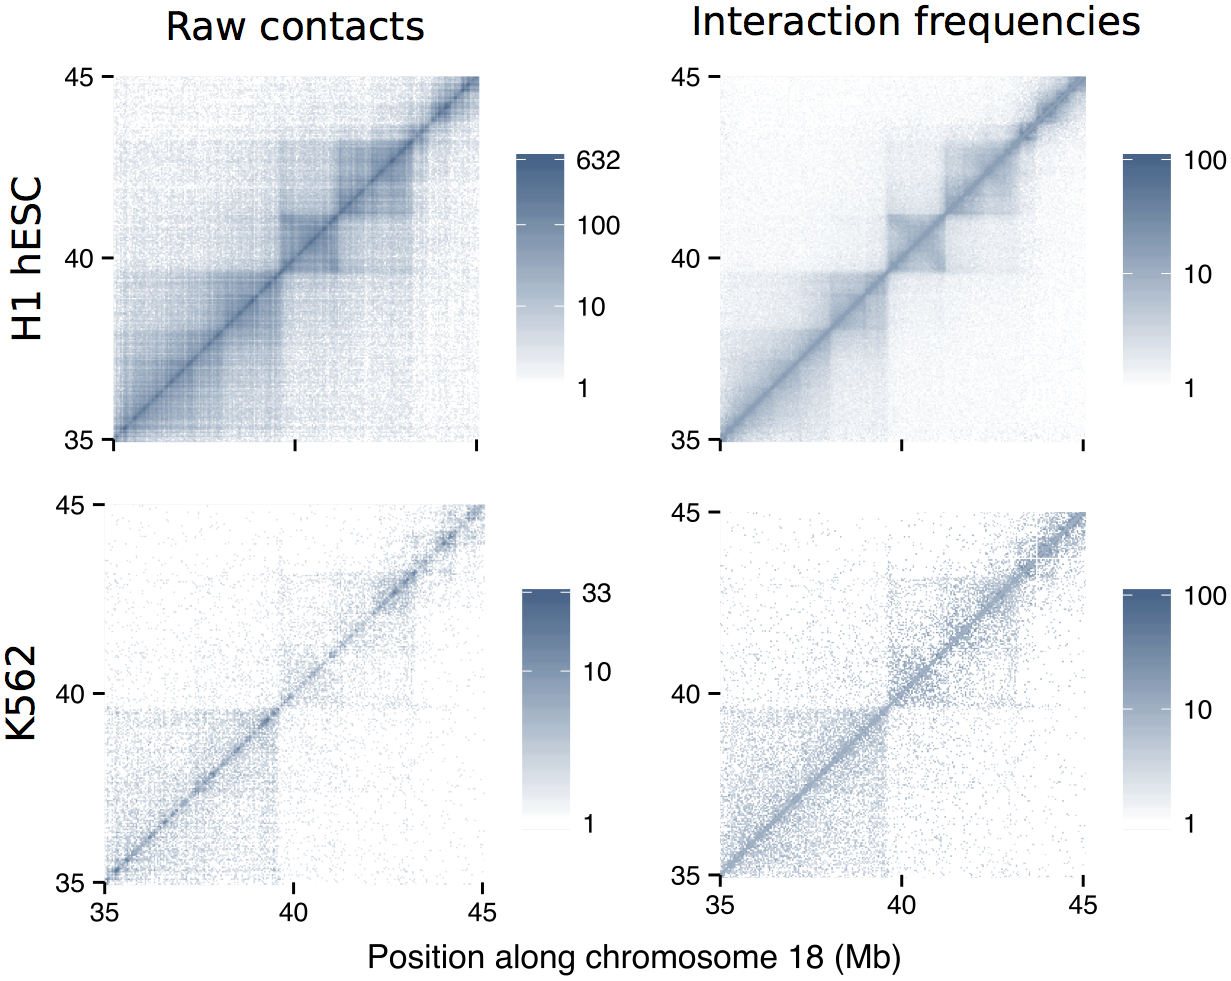
\includegraphics[width=4in]{hicnorm.png}
\captionsetup{width=\textwidth}
\caption[Iterative correction converts raw counts to normalised interaction frequencies.]{
{\bf Iterative correction converts raw counts to normalised interaction frequencies. }
The sample with highest sequencing depth (H1 hESC) is shown alongside a sample with much lower sequencing depth (K562) both before and after iterative correction and normalisation procedures were applied (Methods \ref{methods:hic}) at 40 kb resolution for a 10 Mb section of human chromosome 18. Fill gradients are on a $\log_{10}$ scale.
}\label{fig:hicnorm}
\end{center}
\end{figure} 

Figure \ref{fig:hicnorm} shows a 10 Mb region of chromosome 18 before and after filtering and normalisation in two different cell types. Self-interacting domains visible in the deeply-sequenced H1 hESC cell type also become more visible in the K562 cell type after normalisation. In addition many of the long-range and intra-domain contacts visible in each raw contact map are down-weighted during the normalisation procedure, indicating their prominence was enhanced by biases or other sources of noise in the experimental procedure (Fig. \ref{fig:hicnorm}).

The relative sparsity of the K562 Hi-C contact map compared to that of the H1 hESC cell line should also be noted (Fig. \ref{fig:hicnorm}). At the time much of this study was performed, deeply-sequenced Hi-C datasets for cell lines K562 and GM12878 were not available, thus the majority of analyses were performed at a lower resolution of 1 Mb to further reduce the impact of variable sequencing depth between cell lines (Methods \ref{methods:hic}).

\section{Compartment profiles}\label{sec:wiggles}
% how well do compartments correlate

After uniformly reprocessing each Hi-C dataset and calling compartment eigenvector profiles (Methods \ref{sec:eigs}), we can compare these between three human cell lines. We find compartment profiles have a striking concordance (Fig. \ref{fig:wiggles}), despite the variable sources of both sample material and experimental data. This strong correlation of higher order chromatin structure (at the level of compartments) between three very different human cell types shows that the vast majority of genomic regions appear to be constitutively present in either the A or B compartments regardless of cell lineage.

\begin{figure}
\begin{center}
\makebox[\textwidth][c]{ 
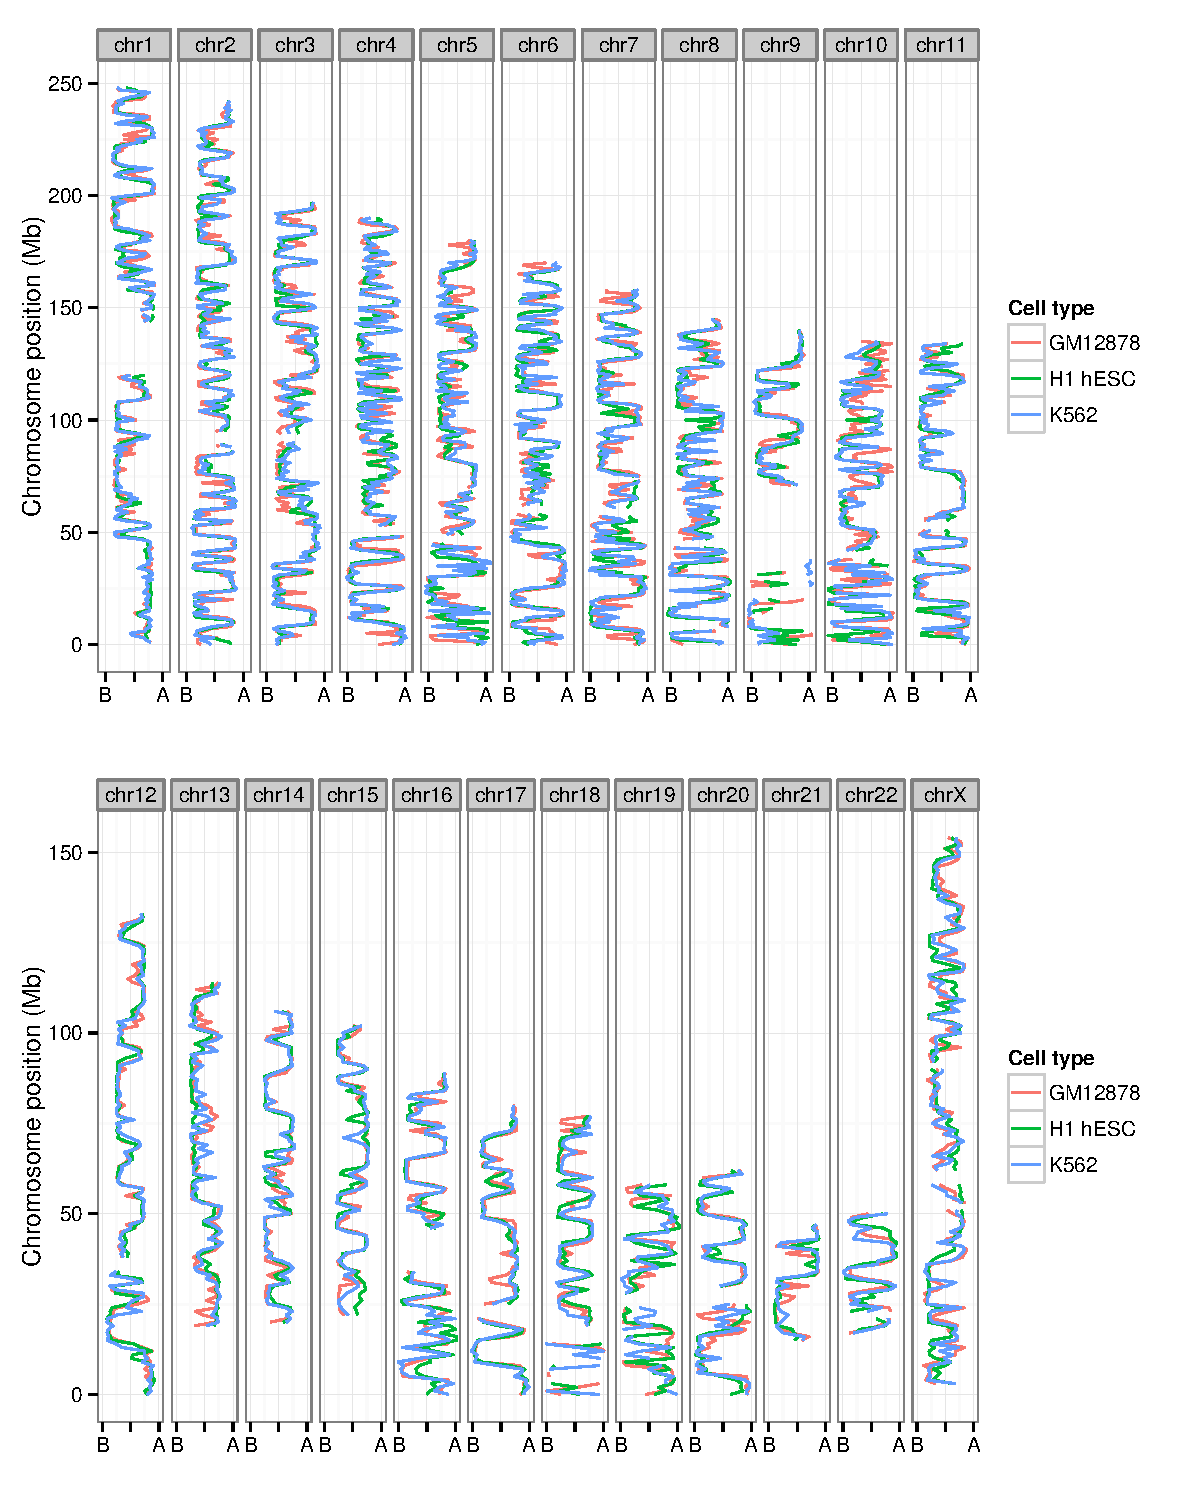
\includegraphics[width=\textwidth]{wiggles.pdf}
}
\captionsetup{width=\textwidth}
\caption[Compartment profiles are observably well-correlated between human cell types and across all chromosomes]{
{\bf Compartment profiles are observably well-correlated between human cell types and across all chromosomes.}
Compartment eigenvectors are plotted along the lengths of each human chromosome (chrY and chrM are omitted). In each case the overlaid profiles show strong concordance between the three different human cell types under study.
}\label{fig:wiggles}
\end{center}
\end{figure} 

This close correspondence also validates our approach of combining these different datasets, and suggests our uniform pipeline is successfully accounting for differences in sequencing depth and other batch effects. The pairwise Pearson correlation coefficients between these independent measures are all in the interval $[.75, .8]$ (Fig. \ref{fig:compcor}). Also of note is that each cell type independently shows a similar bimodal distribution of compartment eigenvector, indicative of the two distinct underlying A/B compartment states (Fig. \ref{fig:compcor}).

\begin{figure}
\begin{center}
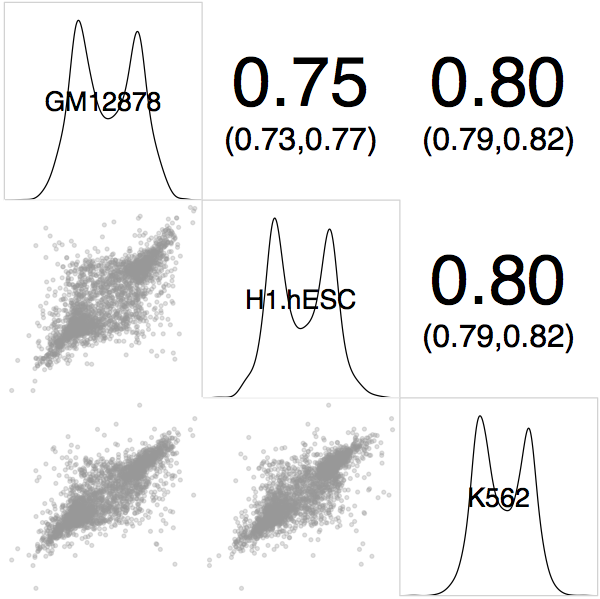
\includegraphics[width=3in]{compartment_corr.png}
\captionsetup{width=\textwidth}
\caption[Compartment eigenvectors are highly correlated between human cell types]{
{\bf Compartment eigenvectors are highly correlated between human cell types.}
Megabase resolution compartment eigenvector values are shown in a plot matrix. \emph{Upper triangle}: Pearson correlation coefficients between pairs, with $95\%$ confidence intervals; \emph{diagonal}: kernel density estimates of eigenvector values per cell type; \emph{lower triangle}: pairwise $x$-$y$ scatterplots of compartment eigenvector values.
}\label{fig:compcor}
\end{center}
\end{figure} 

\section{Domain calls}

\subsection{Compartments}\label{sec:compcalls}

The continuous compartment eigenvector is most commonly used as-is to classify A/B compartments by thresholding based on sign: typically the eigenvector is orientated such that positive values reflect A compartments and negative values B compartments.\cite{Lieberman2009, Kalhor2012} However, given that compartments are understood to be generally broad and alternating domains along a chromosome, often aligning with other large domains such as LADs, an improved classification method might penalise the calls of very short compartment calls, which may be the result of noise. For this reason, instead of using raw eigenvector values we consider observed values as emissions from unobserved underlying states (Fig. \ref{fig:hmmflow}). We built a hidden Markov model (HMM; Methods \ref{meth:hmm}) to represent these states through a well-described probabilistic framework.\cite{Eddy2004}

\begin{figure}
\begin{center}
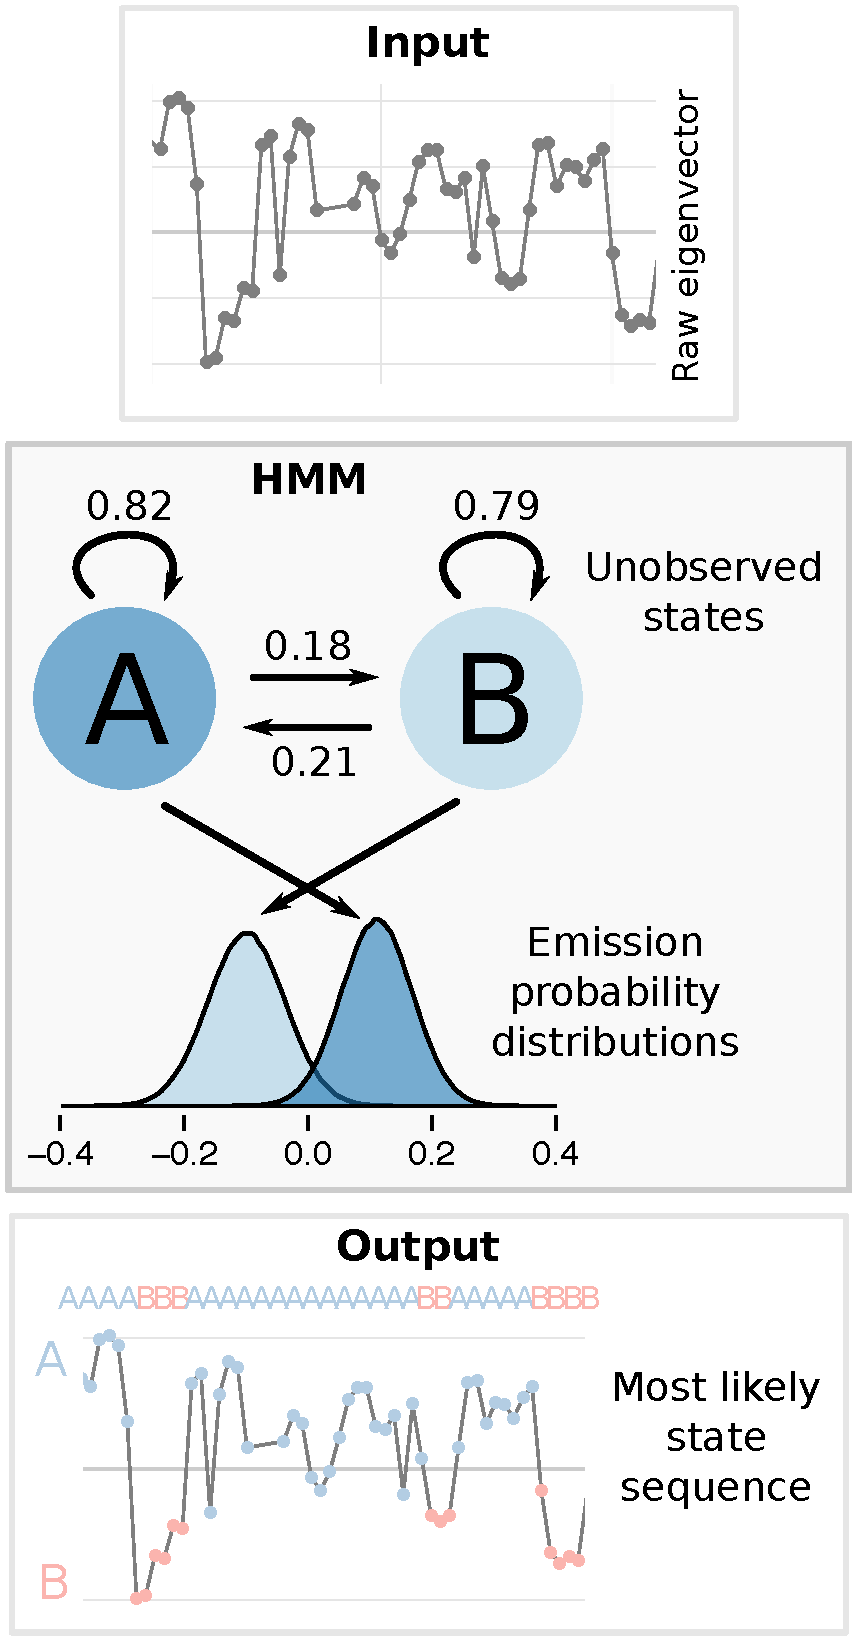
\includegraphics[width=3.2in]{hmm_flow.pdf}
\captionsetup{width=\textwidth}
\caption[ Overview of HMM method for compartment calls.  ]{ {\bf Overview of HMM method for compartment calls.  }
Schematic of HMM method for compartment calls, showing transition probabilities and emissions distributions learned in the GM12878 cell type. A description of HMMs is given in Methods \ref{meth:hmm}. Emission distributions for each cell type are shown in Figure \ref{fig:hmmdist}.
}\label{fig:hmmflow}
\end{center}
\end{figure} 

 Firstly we designed the HMM to have two unobserved states with univariate Gaussian distributed emissions (representing our A and B compartments; Fig. \ref{fig:hmmdist}). To parameterise these states we used the iterative Baum-Welch algorithm, an Expectation-Maximisation procedure designed for HMMs. Having parameterised the HMM for each cell type, we then use the Viterbi algorithm to infer the most likely state sequence to have generated our observed data. This two-state sequence is then used to assign compartment identities to genomic bins. A schematic of this procedure is shown in Figure \ref{fig:hmmflow}.
%This can be modelled through a Hidden Markov Model (HMM), whereby we first parameterise models of state and their transitions, then infer the most likely state sequence to have emitted our observed data (Fig. \ref{fig:hmmflow}). This unobserved two-state sequence is then used for compartment calls (Methods \ref{sec:compartments}). 

\begin{figure}
\begin{center}
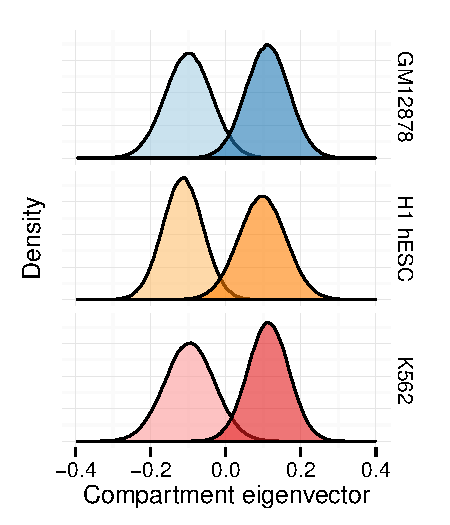
\includegraphics[width=2.75in]{hmm_dists.pdf}
\captionsetup{width=\textwidth}
\caption[ Univariate Gaussian emission distributions for A and B unobserved HMM states. ]{ {\bf Univariate Gaussian emission distributions for A and B unobserved HMM states. }
Probability distributions for compartment eigenvector values per HMM state are shown for each cell type. Distributions centred below zero (lighter colours) show the distribution for the B compartment state, distributions centred above zero (darker) represent the A compartment state.
}\label{fig:hmmdist}
\end{center}
\end{figure} 

In practice, this approach acts to de-noise our compartment calls. Whereas single sign-changes along the series would (under a simple thresholding procedure) have resulted in a single-block compartment, these may now be modelled as noisy emissions from a single unobserved state. An exemplar region is shown in Figure \ref{fig:denoise}. This shows an approximately 50 Mb region from chromosome 8 with eigenvector data from the H1 hESC cell line. A simple thresholding method in this region calls a total of $12$ regions, whereas our HMM method finds only $6$ larger regions in the same window. The disparity is caused by very short and single-bin compartments being disfavoured by the HMM-based method (e.g. Fig. \ref{fig:denoise}). 

\begin{figure}
\begin{center}
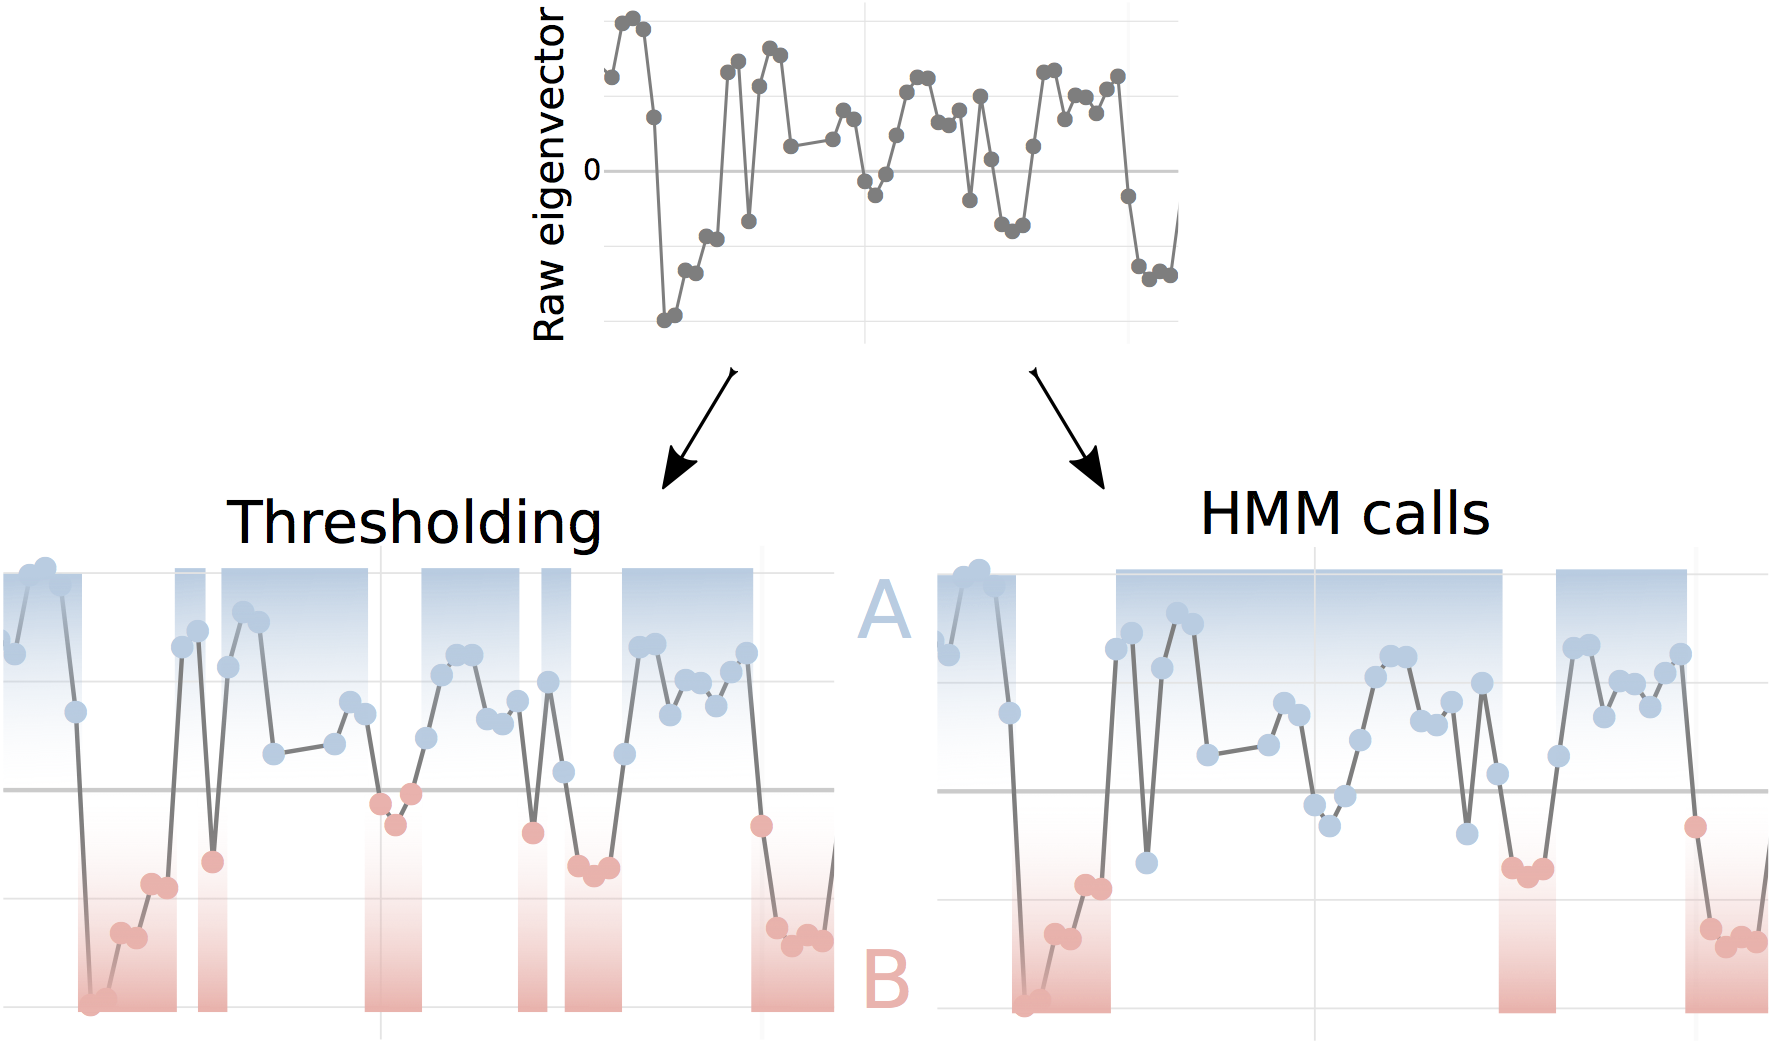
\includegraphics[width=4.5in]{hmm_calls.png}
\captionsetup{width=\textwidth}
\caption[Compartment calls by simple thresholding method or context-aware HMMs.]{ {\bf Compartment calls by simple thresholding method or context-aware HMMs.}
Chromosome compartments have previously been called through simple thresholding at $0$,\cite{Lieberman2009} in this work we use a novel HMM-based method to call unobserved states that have emitted our noisy observed values (\emph{right}).
}\label{fig:denoise}
\end{center}
\end{figure} 

Having called compartments we can compare their properties across cell types. In each case, a majority of chromosome compartment sizes are in the range $0$--$10$ Mb, with a handful of compartments reaching up to $40$ Mb in size (Fig. \ref{fig:compsizedists}). Median sizes for compartments called in this work match those reported previously, with a median size of around $5$ Mb.\cite{Dekker2013} Our slightly larger mean compartment sizes (up to $7.6$ Mb in H1 hESC) may be due to our altered domain calling procedure (Fig. \ref{fig:denoise}) and is clearly influenced by some large outliers (Fig. \ref{fig:compsizedists}).

\begin{figure}
\begin{center}
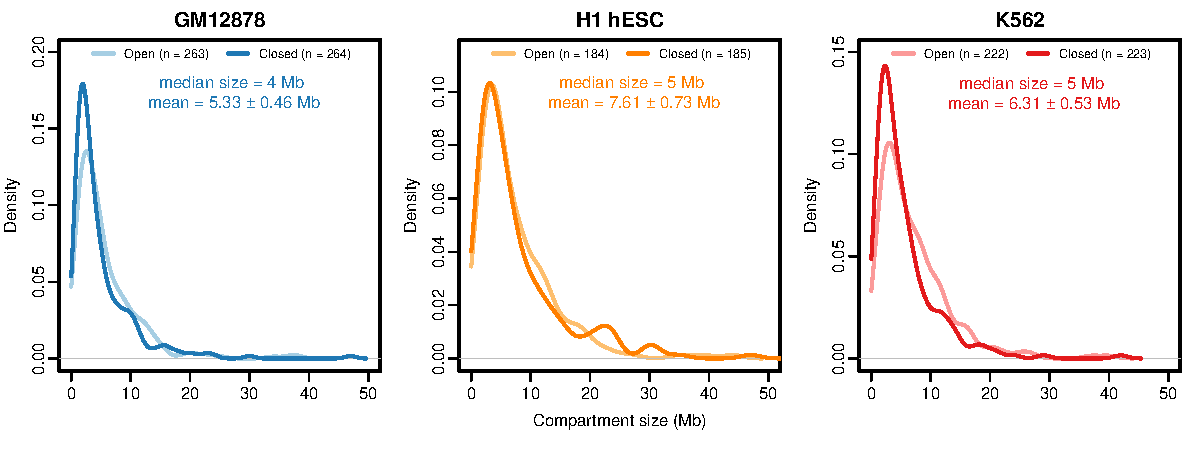
\includegraphics[width=5.8in]{comp_sizedists.pdf}
\captionsetup{width=\textwidth}
\caption[ Size distributions of compartments called in three human cell types. ]{ {\bf Size distributions of compartments called in three human cell types. }
Kernel density estimates of compartment sizes (Open: A; Closed: B) are shown per cell type with summary statistics (\emph{inset}), including mean compartment size with $95\%$ confidence intervals.
}\label{fig:compsizedists}
\end{center}
\end{figure} 

Next we compare compartments between the three cell types under study. To do this, we calculate the minimum absolute distance from each boundary in one cell type against those in a designated comparison cell type (we used H1 hESC). The cumulative distribution of these boundary differences is shown (Fig. \ref{fig:compdist}) and compared to a null distribution of random compartment boundaries (Methods \ref{meth:boundcompare}). We find boundaries are significantly more closely aligned across  cell types than is expected by chance. For example, genome-wide approximately $37\%$ of compartment boundaries in H1 hESC have a corresponding boundary within $100$ kb in GM12878 (and $35\%$ in K562, but only $5\%$ in random boundaries). Comparisons of the cumulative boundary distance distributions yield statistically significant differences relative to the null model (K-S test, K562: $D = 0.47$; $p \approx 0$; GM12878: $D = 0.49$; $p \approx 0$; Fig. \ref{fig:compdist}).

\begin{figure}
\begin{center}
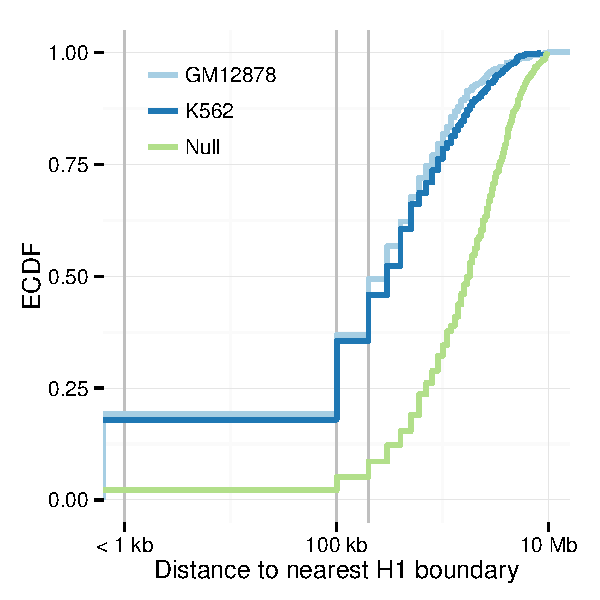
\includegraphics[width=2.5in]{compdist_v2.pdf}
\captionsetup{width=\textwidth}
\caption[Compartment boundaries are shared between cell types. ]{ {\bf Compartment boundaries are shared between cell types. }
The empirical cumulative distribution functions (ECDF) of distances between H1 compartments and those called in GM12878 and K562 are shown. Vertical lines mark distances of 0, 1 and 2 bins. Also plotted is the ECDF of a null model, where distances were calculated to shuffled boundaries at a matched resolution (Methods \ref{meth:boundcompare}).
}\label{fig:compdist}
\end{center}
\end{figure} 

% figure showing size distributions of Hi-C domains
\subsection{TADs}\label{sec:calledtads}

Topological associating domains (TADs) are self-interacting blocks of the genome first described by \citet{Dixon2012} We applied the original TAD calling method without modification, which uses a measure of the directional contact bias of a fragment (Section \ref{intro:tads} and Fig. \ref{fig:dicalc}).

% figure with number of tads per cell type
\begin{figure}
\begin{center} 
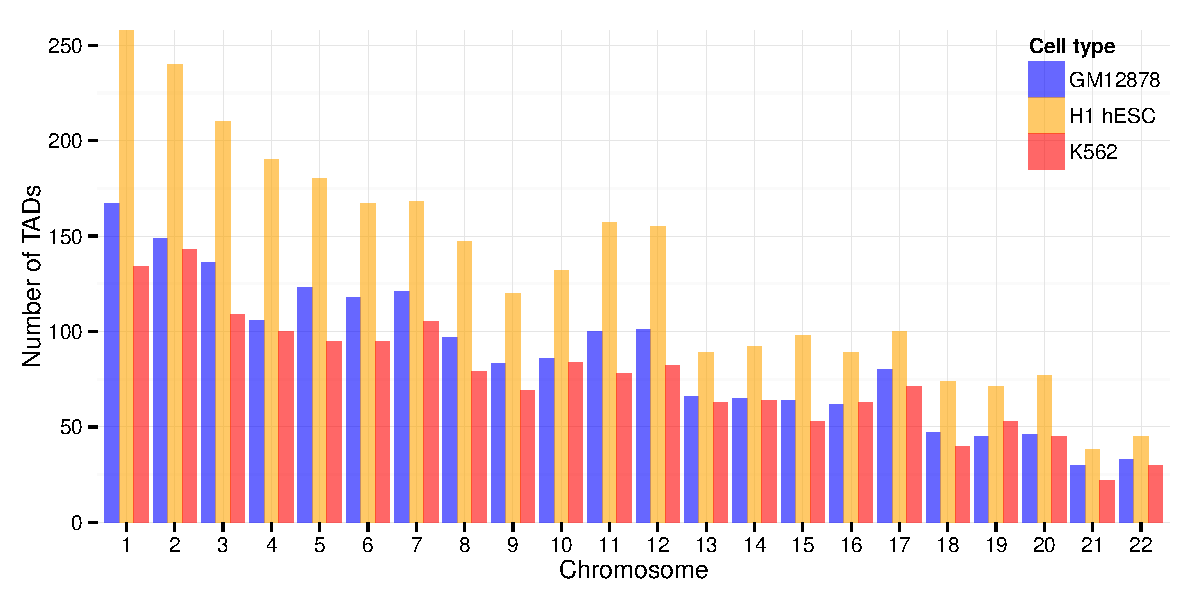
\includegraphics[width=5in]{ntads.pdf}
\captionsetup{width=\textwidth} 
\caption[The number of TADs called per chromosome in each cell type under study.]{ {\bf The number of TADs called per chromosome in each cell type under study. }
A greater number of TADs were called in H1 hESC ($2,897$ total) than in GM12878 ($1,925$) or K562 ($1,677$), due to the difference in sequencing depths in each experiment when matrices were binned at 40 kb resolution.
}\label{fig:ntads}
\end{center} 
\end{figure} 

The \citet{Dixon2012} method of calling TADs relies on the detection of boundaries,\cite{Rao2014} thus it is affected by sequencing depth: experiments with sparser contact matrices may not contain enough for a sufficiently high degree of bias to allow a boundary call. This is evident in our datasets even after normalisation, with the deeply-sequenced H1 hESC cell type having approximately $50\%$ more TADs called than in the GM12878 cell type (Fig. \ref{fig:ntads}). The increased power to detect TAD boundaries also results in smaller domains, on average, in the H1 hESC cell line (Fig. \ref{fig:tadsizes}). This effect could have been mitigated by down-sampling reads in the H1 cell type, but at a cost of reducing the quality of the best dataset under study. Instead this disparity should just be noted as a potential cofounder in downstream TAD analysis; at lower-resolution such as that used to calculate compartment eigenvectors (1 Mb) this sensitivity to sequencing depth is not evident (Figs. \ref{fig:wiggles}, \ref{fig:compcor}).

\begin{figure}
\begin{center}
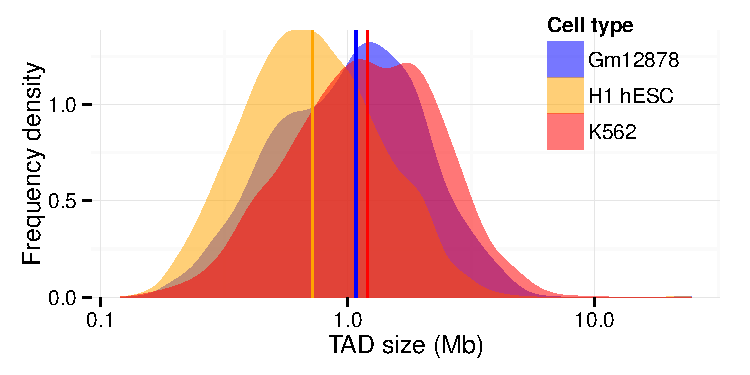
\includegraphics[width=3.1in]{tadsizes.pdf}
\captionsetup{width=\textwidth}
\caption[ Size distributions of TADs called in three human cell type. ]{
{\bf Size distributions of TADs called in three human cell type. }
Densities of TAD sizes called in each cell type under study. Vertical lines show the median TAD size in each cell type (Gm12878: $1.08$ Mb; H1 hESC: $0.72$ Mb; K562: $1.2$ Mb). Sizes distributions shown on a $\log_{10}$ scale.
}\label{fig:tadsizes}
\end{center}
\end{figure} 

Despite differing numbers, there is still detectable levels of conservation of TADs between cell types (Fig. \ref{fig:bounddist}). Genome-wide, $45\%$ of all H1 TAD boundaries have a matching boundary in GM12878 in the same or an adjacent 40 kb bin (K562: $41\%$, null model: $22\%$; K--S test: $D=0.2$, $p\approx0$). To illustrate this conservation with a real example, a 20 Mb region of chromosome 2 is pictured (Fig. \ref{fig:blowout}), highlighting the conservation between both TADs and compartment calls across the three cell types and at multiple scales: from chromosome-wide 1 Mb compartment eigenvectors, to TADs with individual boundaries resolved to 40 kb.

\begin{figure}
\begin{center}
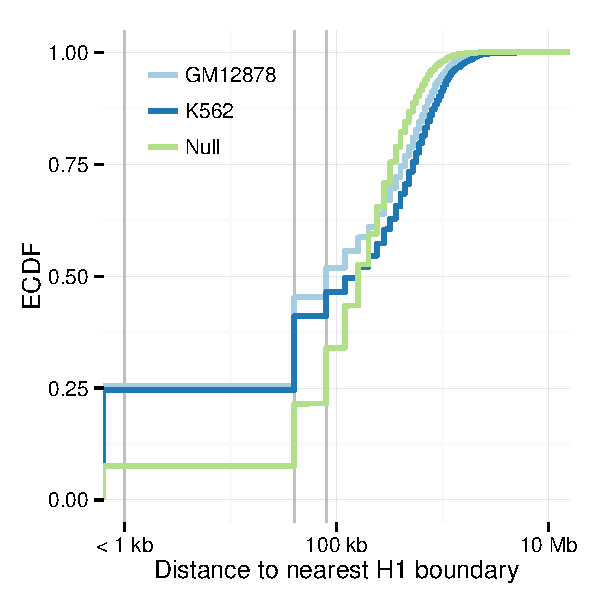
\includegraphics[width=2.5in]{taddist_v2.pdf}
\captionsetup{width=\textwidth}
\caption[TAD boundaries are shared between cell types. ]{ {\bf TAD boundaries are shared between cell types. }
The empirical cumulative density functions (ECDF) of distances between H1 TADs and those called in GM12878 and K562 are shown. Vertical lines mark distances of 0, 1 and 2 bins. Also plotted is the ECDF of a null model, where distances were calculated to shuffled boundaries at a matched resolution (Methods \ref{meth:boundcompare}).
}\label{fig:bounddist}
\end{center}
\end{figure} 

\begin{figure}
\begin{center} 
\makebox[\textwidth][c]{ 
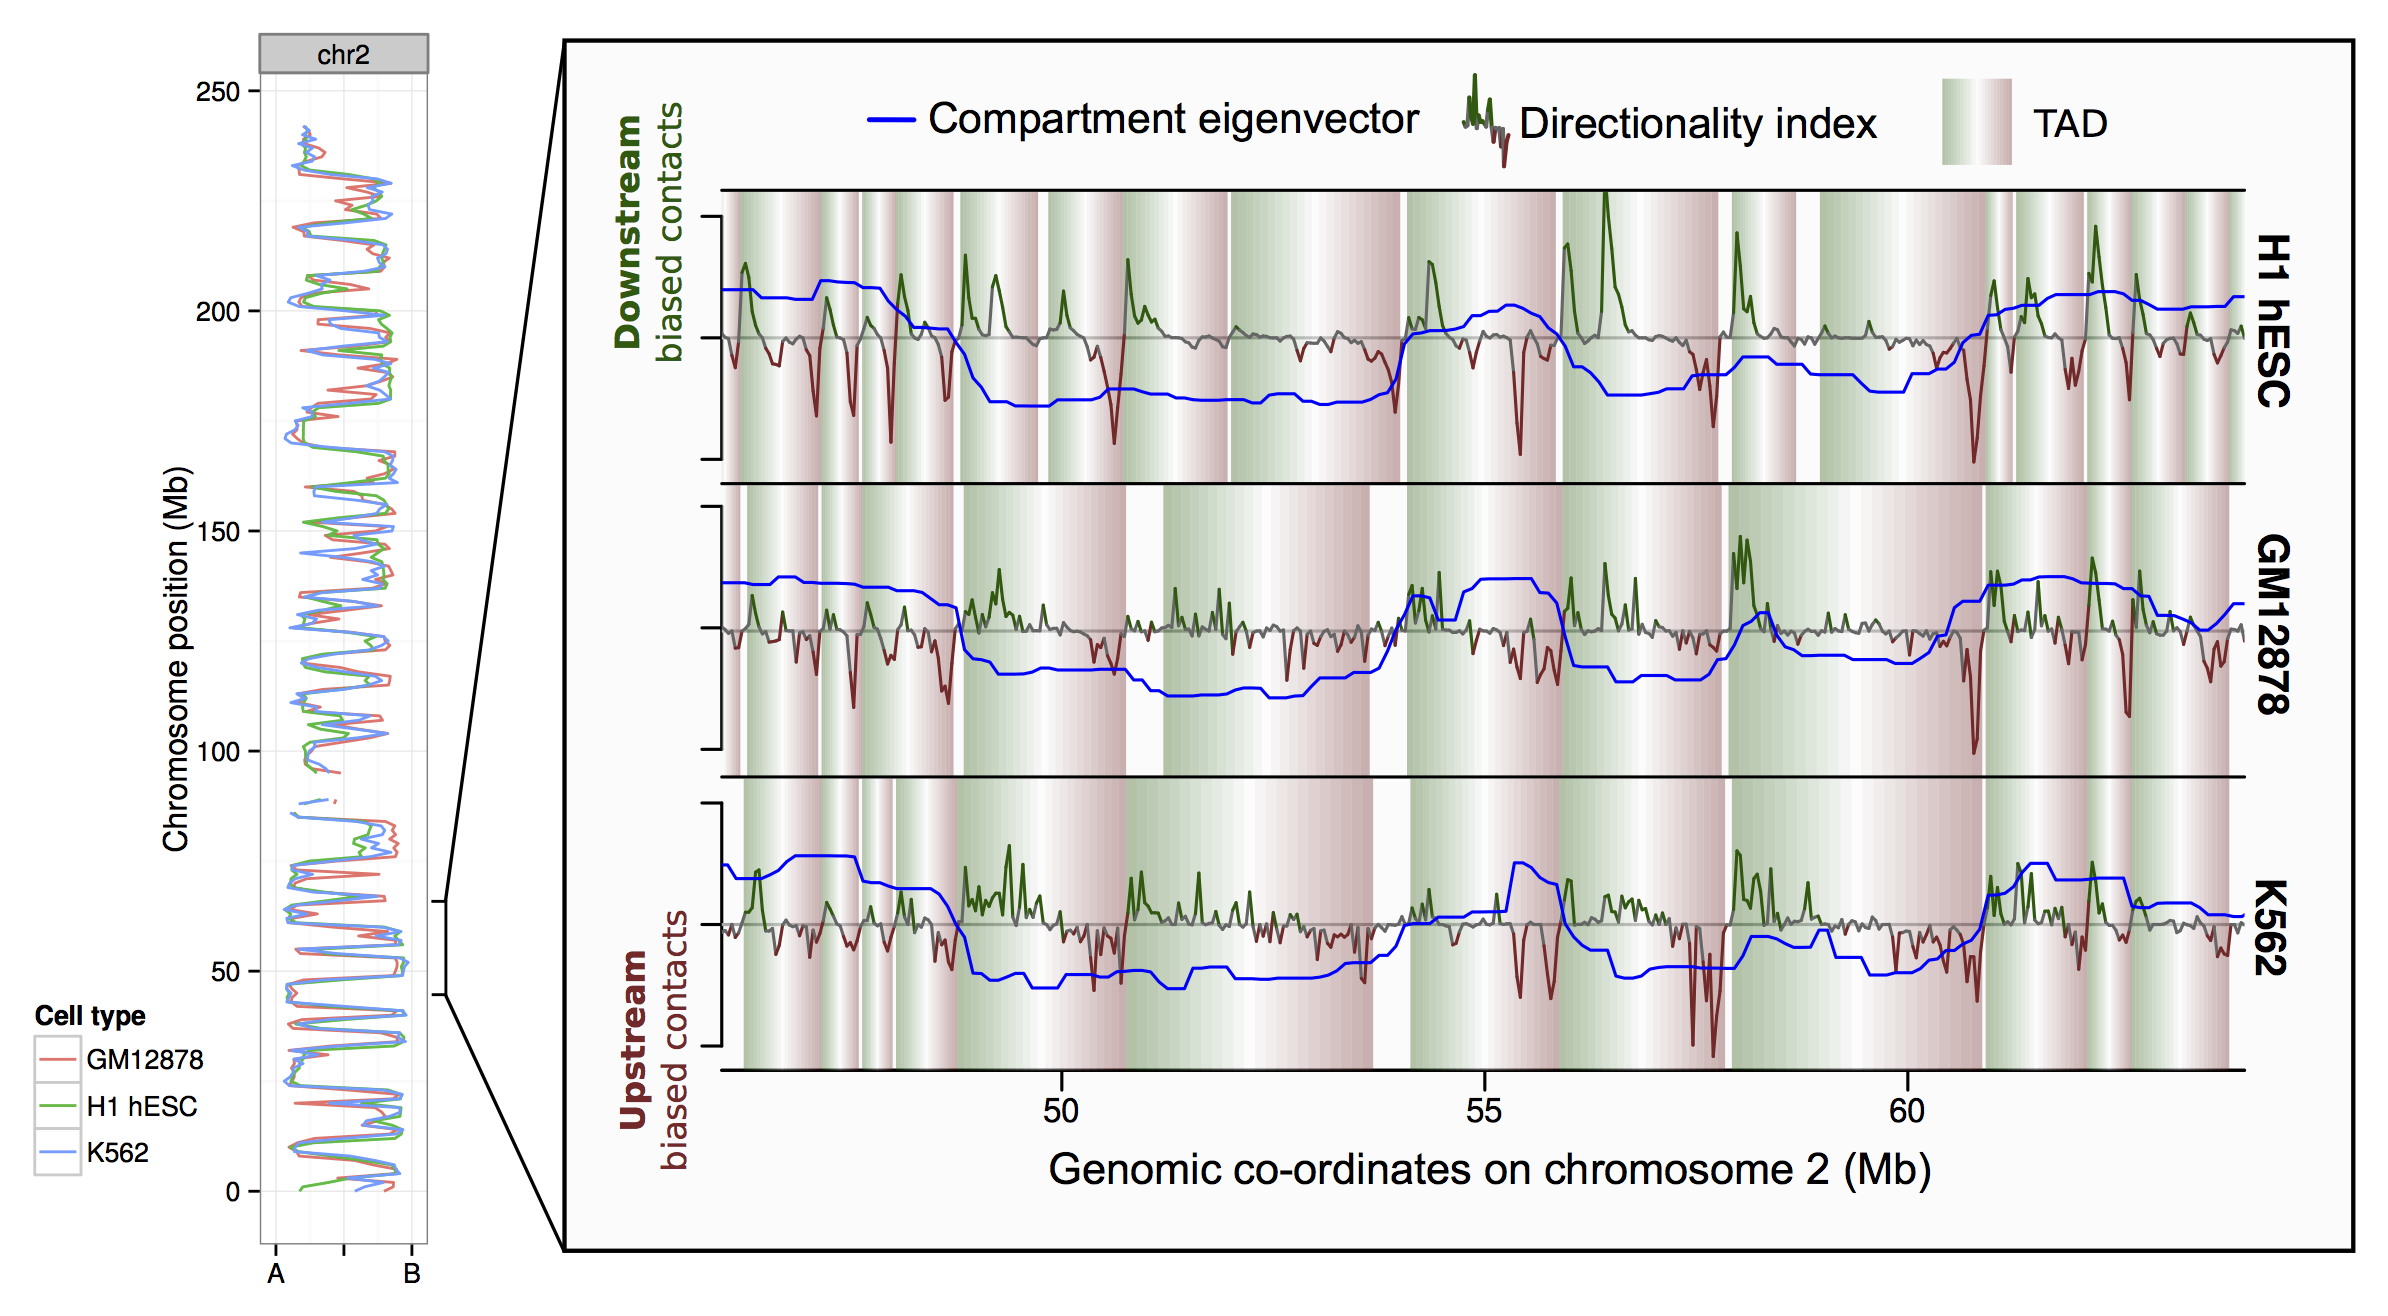
\includegraphics[width=\textwidth]{blowout.png}
}
\captionsetup{width=\textwidth} 
\caption[Concordance of chromatin structure at multiple scales over three human cell types.]{ {\bf Concordance of chromatin structure at multiple scales over three human cell types. }
The eigenvector compartment profile is shown for chromosome 2 for three human cell types (\emph{left}).  At higher resolution, the zoomed region illustrates conservation of topologically associating domains (TADs) over 20 Mb of the same chromosome.
}\label{fig:blowout}
\end{center} 
\end{figure} 

\section{Domain epigenomics}

The use of well-studied human cell types allows intersection with publicly-available epigenomics datasets, such as those produce by the ENCODE consortium.\cite{Dunham2012} In total, 35 cell-matched ChIP-seq datasets were available for all three of the tier 1 ENCODE cell lines: GM12878, H1 hESC and K562 (see Methods \ref{methods:encode}). In this section we integrate reprocessed Hi-C data and derived higher order domains with these various high-resolution datasets.

\subsection{A/B compartments}

The overwhelming majority of intersected chromatin features are significantly enriched in active A compartments relative to B compartments (Fig. \ref{fig:compencode}). This is expected since A compartments represent the actively-transcribed and accessible portions of the genome, and have previously been shown to positively correlate with many of the features shown.\cite{Lieberman2009, Dekker2013}

\begin{figure}
\begin{center}
\makebox[\textwidth][c]{ 
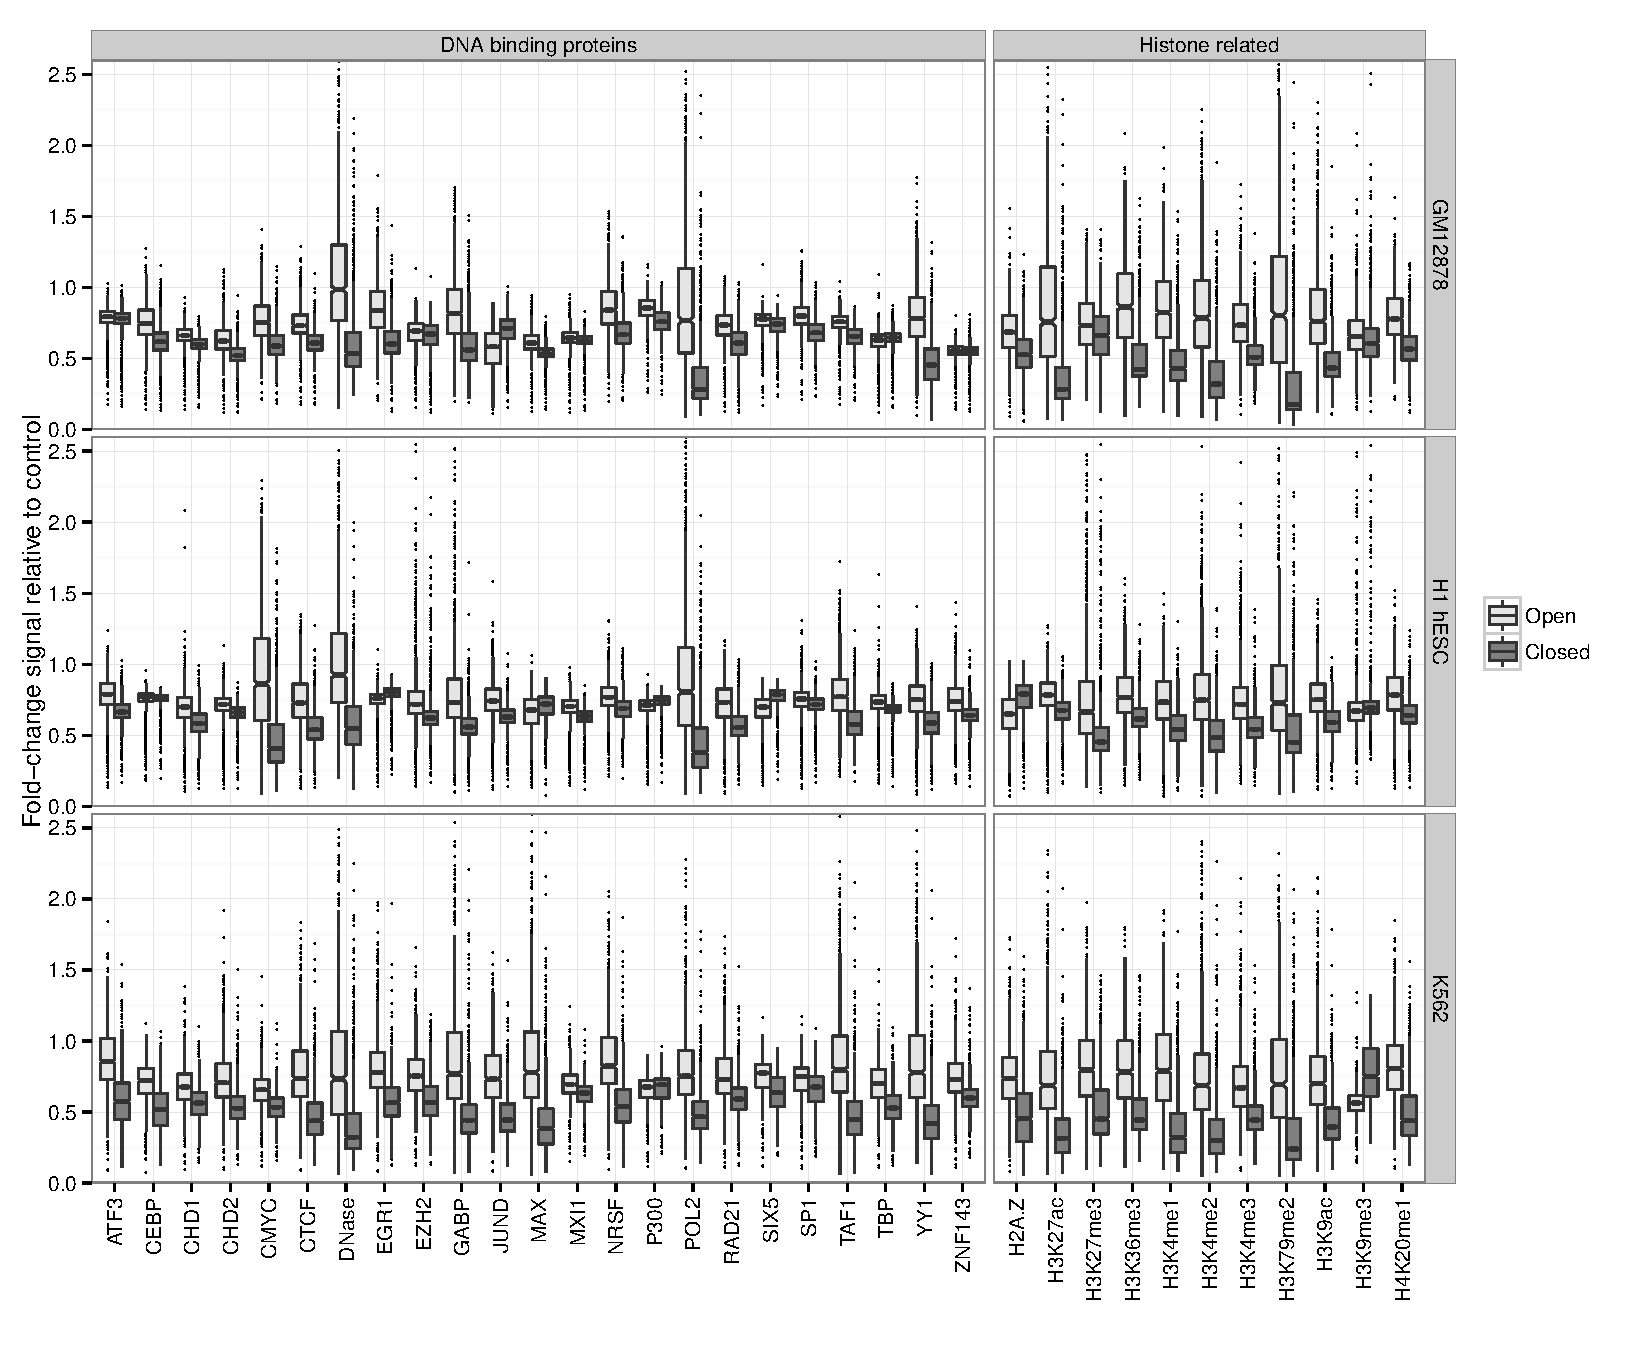
\includegraphics[width=1.1\textwidth]{compartment_encode.pdf}
}
\captionsetup{width=\textwidth}
\caption[The chromatin signatures of A/B compartments.]{ {\bf The chromatin signatures of A/B compartments. }
Notched boxplots summarise the distribution of each feature over 1 Mb bins in open (A) and closed (B) compartments genome-wide.
}\label{fig:compencode}
\end{center}
\end{figure} 

Exceptions to this rule are few. However the repressive histone modification H3k9me3 is found more often in B compartments in two cell types, as is the P300 transcription factor (Fig. \ref{fig:compencode}). Also of note is the histone variant H2A.Z which is significantly enriched in A compartments in GM12878 and K562, but this relationship is reversed in the embryonic stem cell line (Fig. \ref{fig:compencode}). Recent evidence suggests specialised roles for H2A.Z in regulating both repression and activation during embryonic stem cell differentiation, acting as a ``general facilitator''.\cite{Hu2013b} Additionally H2A.Z has been reported to mark histone octamers for depletion, thereby permitting gene activation during differentiation.\cite{Li2012} Potentially, then, the H2A.Z enrichment in B compartments could be driven by regions soon to be de-repressed as the stem cell differentiates.

\subsection{TAD classes}

Unlike compartments, initially TADs were not thought to be correlated with blocks of chromatin features.\cite{Dixon2012} Later studies have linked TADs with such enrichments, first in \emph{Drosophila}\cite{Sexton2012} and later in human cells, where it was argued TADs are merely a low-resolution window to smaller "sub-compartments", bearing similar active and inactive marks to their much-larger namesakes.\cite{Rao2014} Here we look for evidence that TADs called in our human cell types correspond to the "epigenomic domains" identified in \emph{Drosophila} by \citet{Sexton2012} Epigenomic domains were identified through supervised clustering of "physical domains" (TAD analogues called in \emph{Drosophila}) by their average enrichment for selected epigenomic features of known function, for example enrichment of H3K27me3 mark was used to call Polycomb (PcG) associated domains. 

\begin{figure}
\begin{center}
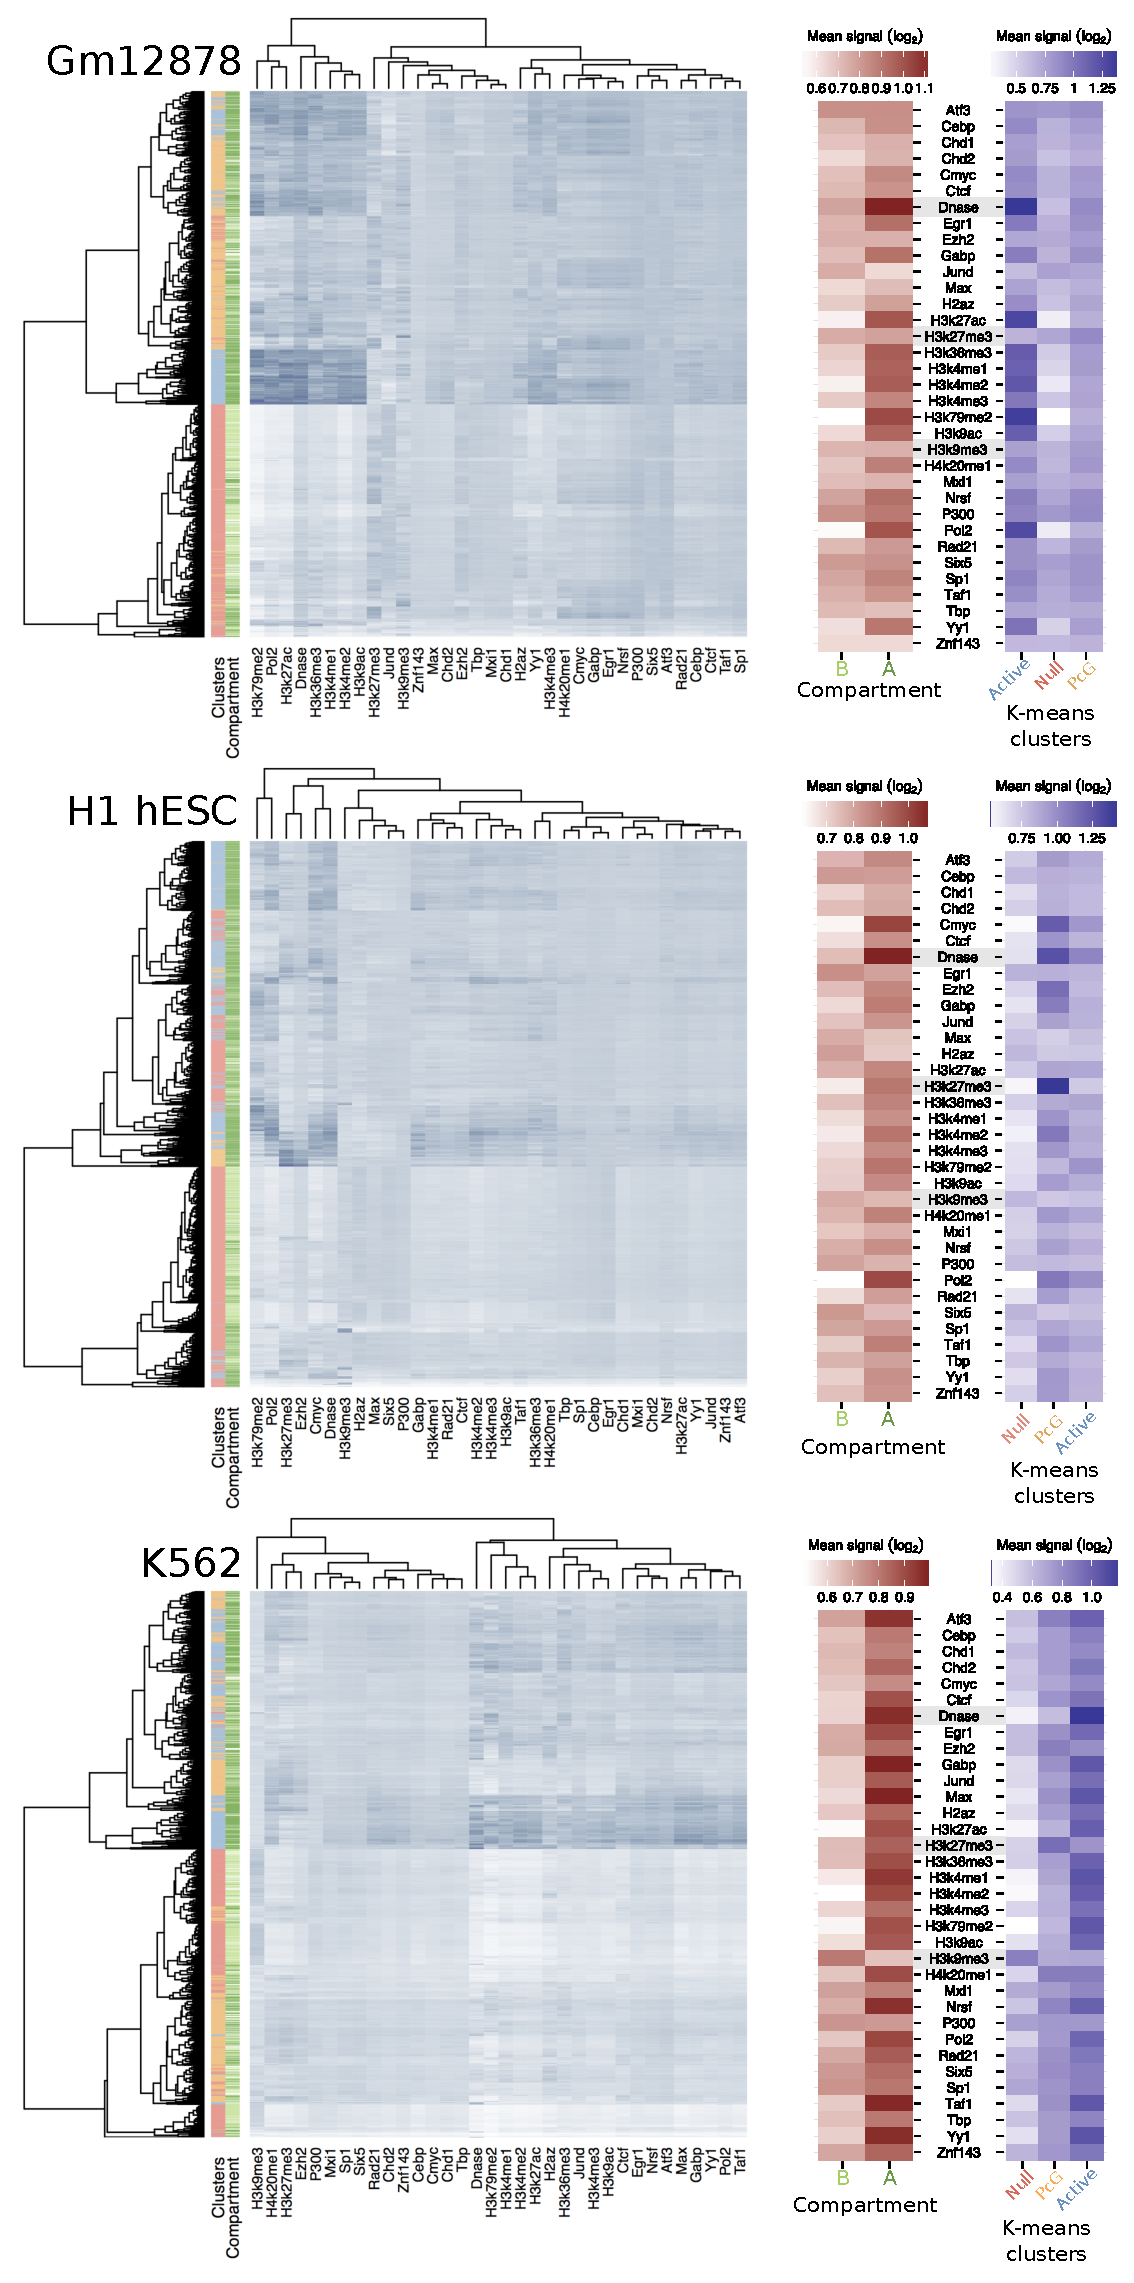
\includegraphics[width=4.5in]{tads_encode.pdf}
\captionsetup{width=\textwidth}
\caption[TADs reflect epigenomic domains.]{ {\bf TADs reflect epigenomic domains. }
Following the \emph{Drosophila} results of \citet{Sexton2012}, clustering of TAD domains by mean $\log_2$ signal of 34 ENCODE features distinguishes �null�, �active� and polycomb-associated (PcG) domains, as well as reflecting the encompassing A/B compartments.
}\label{fig:tadencode}
\end{center}
\end{figure} 

We found that TADs called across the three cell types used in this work could similarly be clustered into transcriptionally active (active), repressed heterochromatin (null) and polycomb-associated (PcG) domains, based on the patterns of DNase hypersensitivity, H3k9me3 and H3k27me3, respectively (Fig. \ref{fig:tadencode}). \emph{Drosophila} physical domains were clustered into four categories, with three of those matching our annotations. The fourth \emph{Drosophila} domain type was enriched for the HP1 protein (therefore likely centromeric) for which we did not have ENCODE ChIP-seq data in all human cell types under study. 

This analysis reveals that active compartments typically cover both active and PcG-associated TADs, while B compartments appear more homogeneous and are composed mostly of H3k9me3-enriched heterochromatin even when considering fine-grained TAD structures rather than megabase-sized genomic blocks (Fig. \ref{fig:tadencode}).

These findings also link with recent work that suggested TADs are windows into ``sub-compartments"\cite{Rao2014} which more closely reflect the functional enrichments of compartments. However, in our data we did not find statistical support for the suggested 5 classes of sub-compartment; instead, an ensemble of algorithms for optimising the number of cluster centroids voted for two or three clusters of TADs (Fig. \ref{fig:nbclust}). This is not wholly surprising as \citet{Rao2014} report sub-compartments only on extremely deep-sequenced samples, and at a scale of organisation below that of TADs.

\section{Variable regions}\label{sec:variableregions}
% investigate those regions which are "flipped"

Despite the vast majority of the genome being in matched chromatin compartments across human cell types (Fig. \ref{fig:wiggles}), there are also regions of disagreement. Reasons for observable differences include technical errors and biases, but also more interesting functional explanations, where cell-type specific activation or repression is reflected in changes in higher order structure.

To conservatively call regions of variable structure (RVS), we used HMM-called compartment states and selected those which were either: i) open in one cell type and closed in both others or ii) closed in one cell type and open in both others. This left sets of RVS which could be considered as "flipped open" or "flipped closed" in a given cell type.

\begin{figure}
\begin{center} 
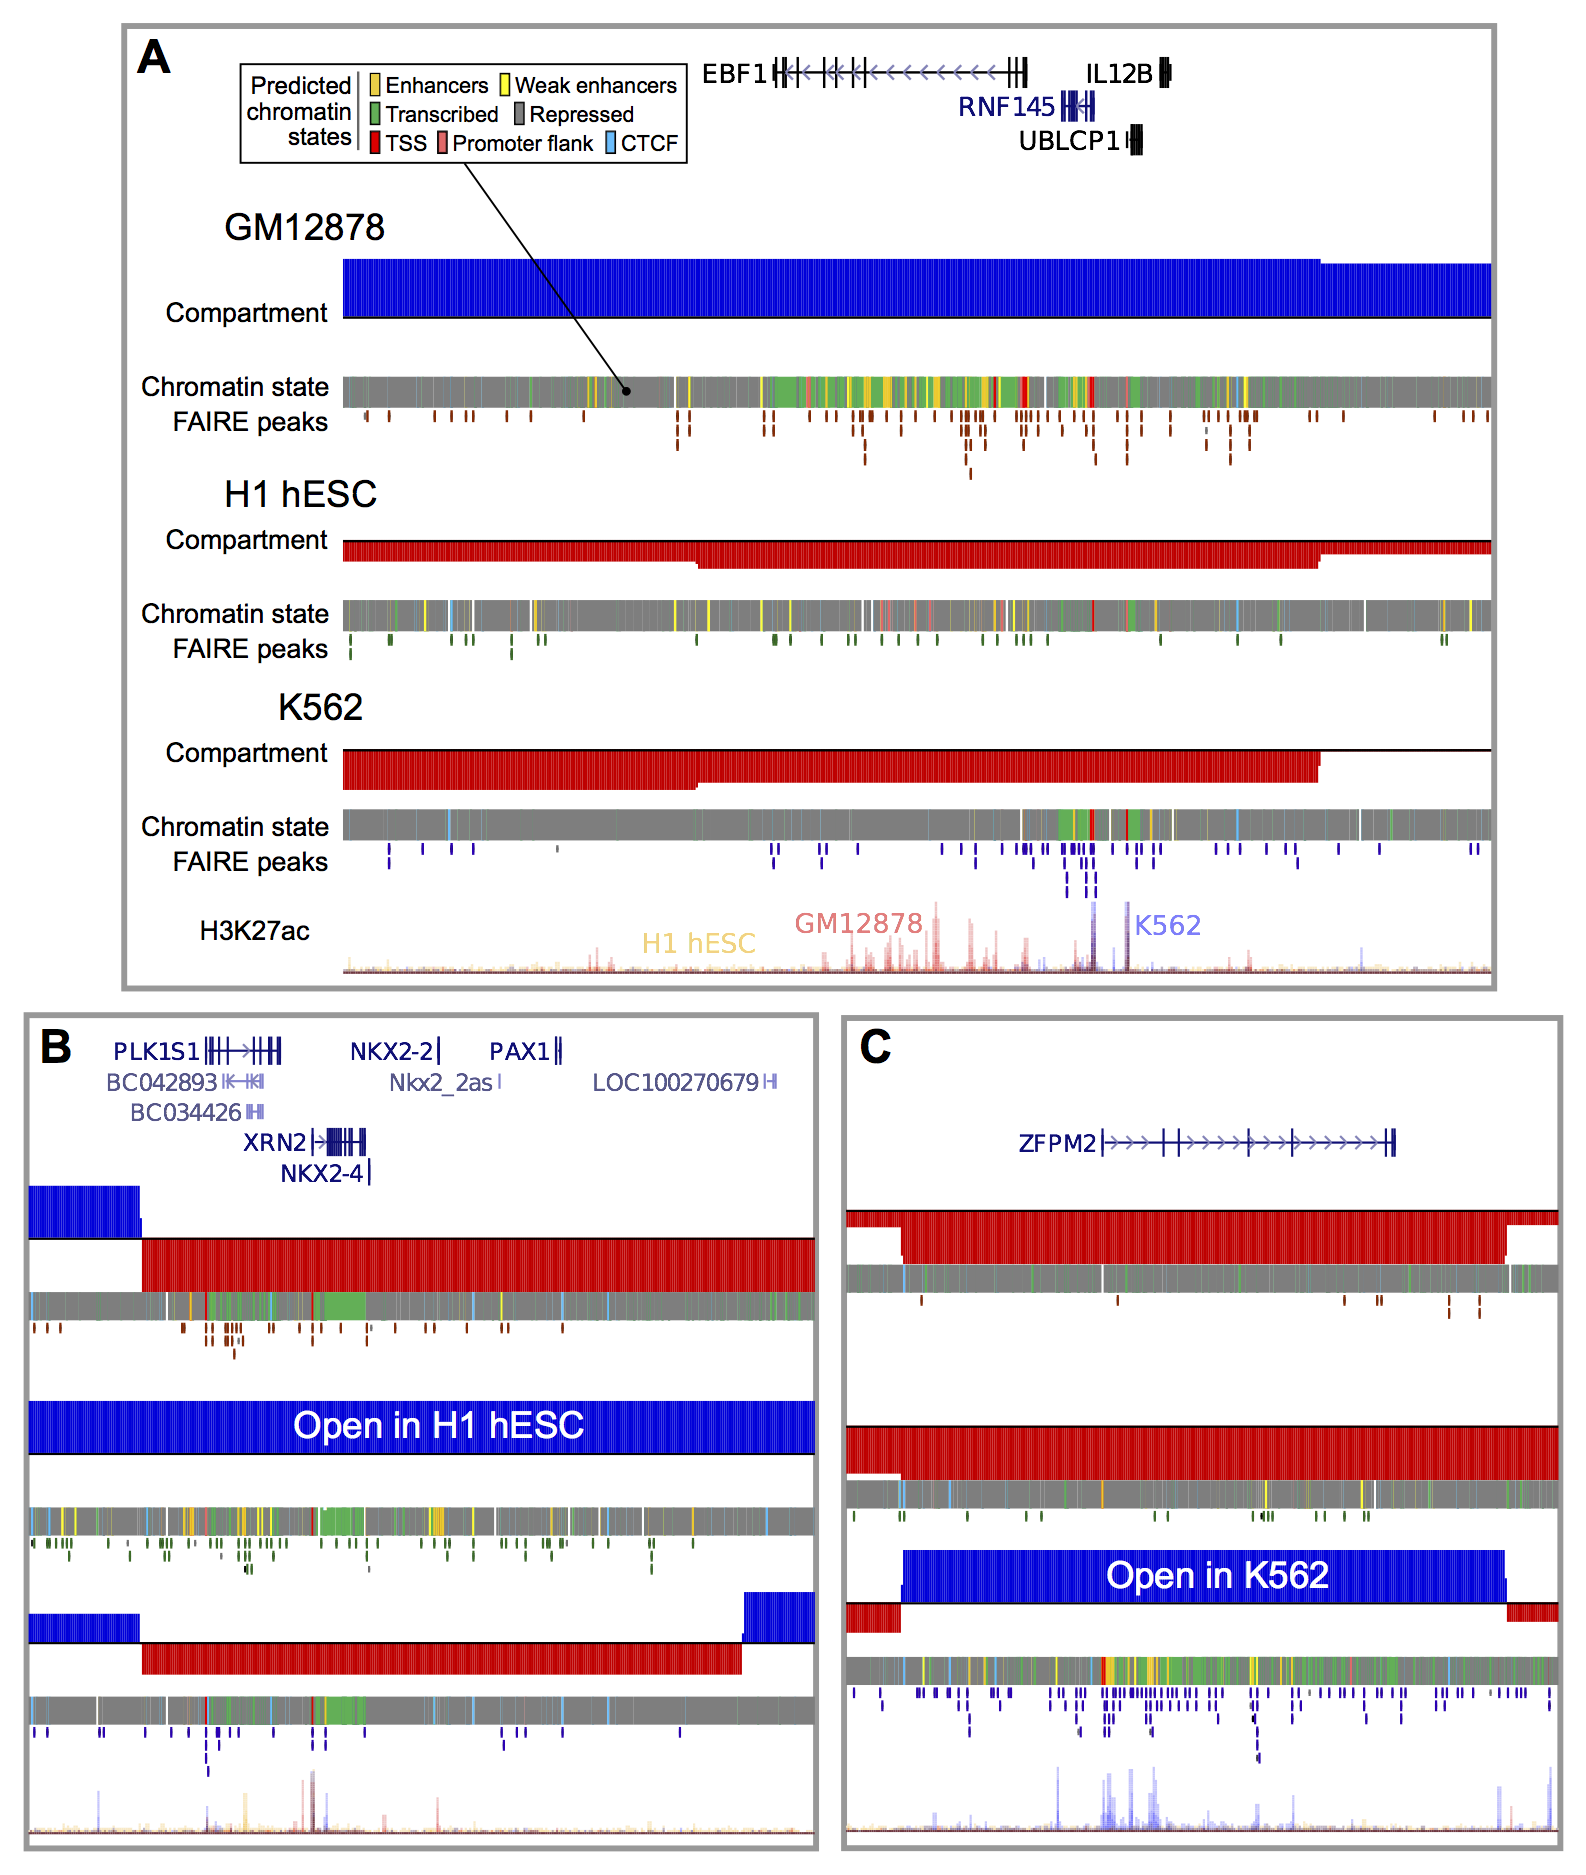
\includegraphics[width=4.5in]{examplervs.png}
\captionsetup{width=\textwidth} 
\caption[Structurally variable regions indicate cell type specific biology.]{ {\bf Structurally variable regions indicate cell type specific biology. } 
Regions occupying the active A nuclear compartment in one cell type, but the repressive B compartment in the other two, were selected and ranked by the number of predicted active enhancers. Examples of particular interest from the top 5 regions per cell type are shown: (A) the chr5:158-159 Mb region which occupies the open A compartment in GM12878 cells, (B) the chr20:21-22 Mb region which is open in H1 hESC, (C) the chr8: 106-107 Mb region which is open in K562. Displayed tracks are: known (UCSC) genes, compartment eigenvectors, chromHMM/Segway combined chromatin state predictions, open chromatin FAIRE peaks, and H3K27ac signal.  
}\label{fig:flippedegs}
\end{center} 
\end{figure} 

% fig 1.
\subsection{Chromatin state enrichment}\label{sec:chromstateenrich}

Given our conservative definition of RVS (Section \ref{sec:variableregions}), such notable changes between transcriptionally permissive and repressive environments might be expected to be associated with cell-type-specific biology, such as functional chromatin states. To test this, we used consensus predicted chromatin state annotations, built from two machine learning algorithms, \texttt{ChromHMM}\cite{Ernst2012} and \texttt{SegWay}\cite{Hoffman2012, Hoffman2013}, and tested for enrichment or depletion in our set of RVS (Methods \ref{enhancer-enrichment}).

We found that RVS show a striking enrichment for cell-type specific enhancers in both of our derived cell lines, but not in embryonic stem cells (Fig. \ref{fig:enhancerstates}). This observation is consistent with the undifferentiated embryonic stem-cell type lacking lineage-specific enhancer contacts active in its pluripotent state. The same pattern was not seen for enhancers shared between two or more of the cell types under study. We observed a similar enrichment for cell-type-specific transcription but not for several other chromatin states including promoter activity (Fig. \ref{fig:stateenrich}).

\begin{figure}
\begin{center}
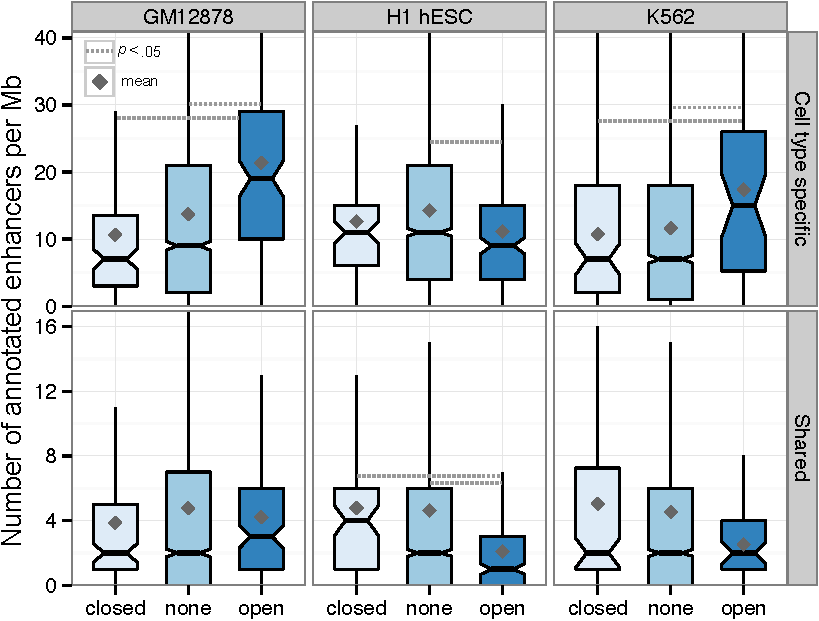
\includegraphics[width=3.5in]{enhancerstates.pdf}
\captionsetup{width=\textwidth}
\caption[Regions of variable structure are enriched for cell type specific enhancers.]{ {\bf Regions of variable structure are enriched for cell type specific enhancers. }
Numbers of predicted enhancer states (cell type specific or shared between two or more cell types) are shown for regions with altered (open or closed) and non-altered (none) compartments in each cell type.
}\label{fig:enhancerstates}
\end{center}
\end{figure} 

Together these state enrichments suggest the identified RVS often reflect functional changes at regions of cell-type specific biology, with heightened enhancer and transcriptional activity in the relevant cell type (Fig. \ref{fig:stateenrich}). Combined with the observed large-scale concordance of higher order chromatin organisation between cell types (Figs. \ref{fig:wiggles}, \ref{fig:blowout}), these results reinforce a model of organisation whereby chromatin organisation is largely conserved and static across cell types, but also permits local flexibility in order to activate or repress regions of biological importance to a given cell type.

\begin{figure}
\begin{center}
\makebox[\textwidth][c]{ 
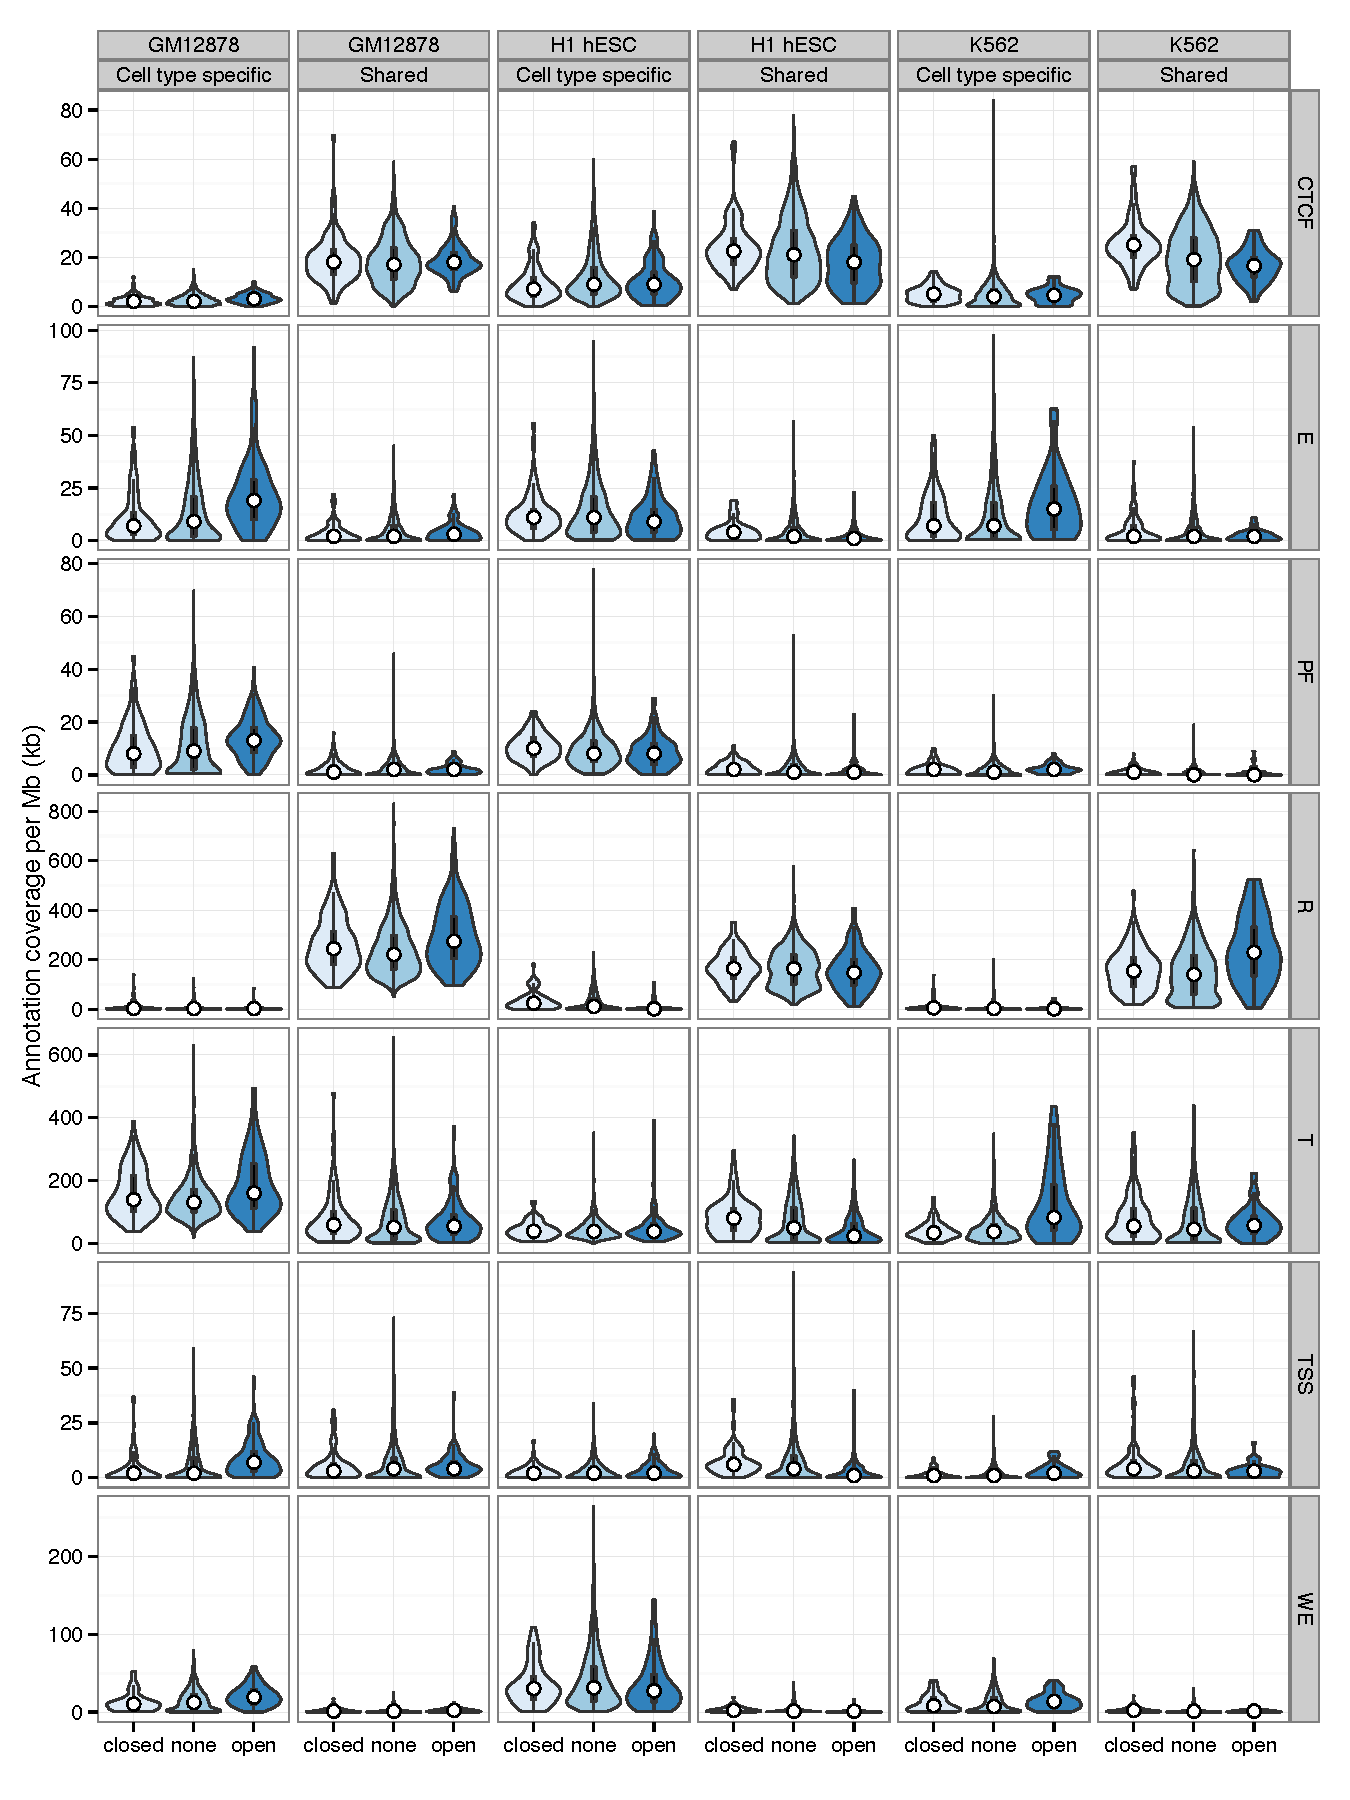
\includegraphics[width=1.1\textwidth]{stateenrich.pdf}
}
\captionsetup{width=\textwidth}
\caption[Distributions of features across all predicted chromatin states in regions of
variable higher order structure.]{ {\bf Distributions of features across all predicted chromatin states in regions of
variable higher order structure. }
Distributions of the average coverage of predicted chromatin states in each Mb per cell type are shown as bean plots. Predicted
chromatin states are those from \citet{Hoffman2013} and are labelled as: TSS: promoter and
TSS; PF: promoter flanking region; E: enhancer; WE: weak enhancer or cis-regulatory element;
CTCF: CTCF enriched element; T: transcribed region; R: repressed or low-activity (Methods \ref{enhancer-enrichment}).
}\label{fig:stateenrich}
\end{center}
\end{figure} 

\subsection{Gene ontology enrichment}

Specific examples of RVS highlight genes of interest (Fig. \ref{fig:flippedegs}) but should be coupled with statistical evidence prior to suggestions of a general trend. For this reason we used Gene Ontology (GO) terms to test for functional enrichment within open RVS per cell type. 

Functional enrichments of genes found in "flipped open" RVS in each cell type were calculated using DAVID \cite{Huang2008, Huang2009} and filtered by false discovery rate (FDR $< .05$; Methods \ref{meth:go}). This revealed slight enrichments for keywords "blood", "oxygen carrier" and "$\beta$ haemoglobin" in the K562 cell type, a multipotent cell type which is known to show properties of an early erythrocyte, among others.\cite{lozzio1981} However, in the other two cell types we did not find significant enrichments across regions, except for artefacts caused by violations of the independence assumption used in GO term hypergeometric testing. Specifically, our RVS blocks were at least 1 Mb each so generally contain more than one gene, thus enrichments were seen for those gene families known to form paralogous clusters along chromosomes, such as olfactory receptors. The full results of these tests are given in the appendix (Tables \ref{tab:gmgo}, \ref{tab:h1go}, \ref{tab:k5go}).

The size of RVS could also explain why we do not capture the relationship hinted at by our cherry-picked examples (Fig. \ref{fig:flippedegs}). Given that regions contain multiple (often unrelated) genes, we can imagine a case where a cell type specific locus is activated and moves into a more central position, disturbing adjacent genes which remain in a repressed state. Thus the cell type specific signals contained within the sum of all RVS in a given cell type could be obscured by the noise of adjacent genes captured in these broad compartment transitions.

\subsection{Contact changes}

A defining characteristic of active A compartment regions is a preferential bias in contacting other A compartment regions.\cite{Lieberman2009} However, it is not clear whether cell-type-specific transitions in higher-order structure are solely compartment-level phenomena, or involve other structural strata. We therefore examined the genome-wide contact profiles of each region of variable cell-type-specific chromatin structure in detail. 

If our cell-type-specific RVS are mediated by finer-scale structural levels (such as TADs) we might expect to see predominantly short-range contact changes in their underlying contact profile. Instead, we found that variable regions preferentially interact with other A compartment regions in the cell types in which they are active (Fig. \ref{fig:longrange}), but not in the other cell types in which they are inactive. This supports the idea that these cell-type-specific regions are undergoing compartment-level transitions, disproportionately mediated by the formation of long-range contacts, while also not precluding additional changes at lower levels such as TADs. Furthermore these contact shifts, particularly when coupled with the observed functional enrichments for transcriptional machinery and enhancer activity (Section \ref{sec:chromstateenrich}), are consistent with active RVS selectively entering into "transcription factories", sites of co-ordinated transcription between potentially distal loci.\cite{Edelman2012}

\begin{figure}
\begin{center} 
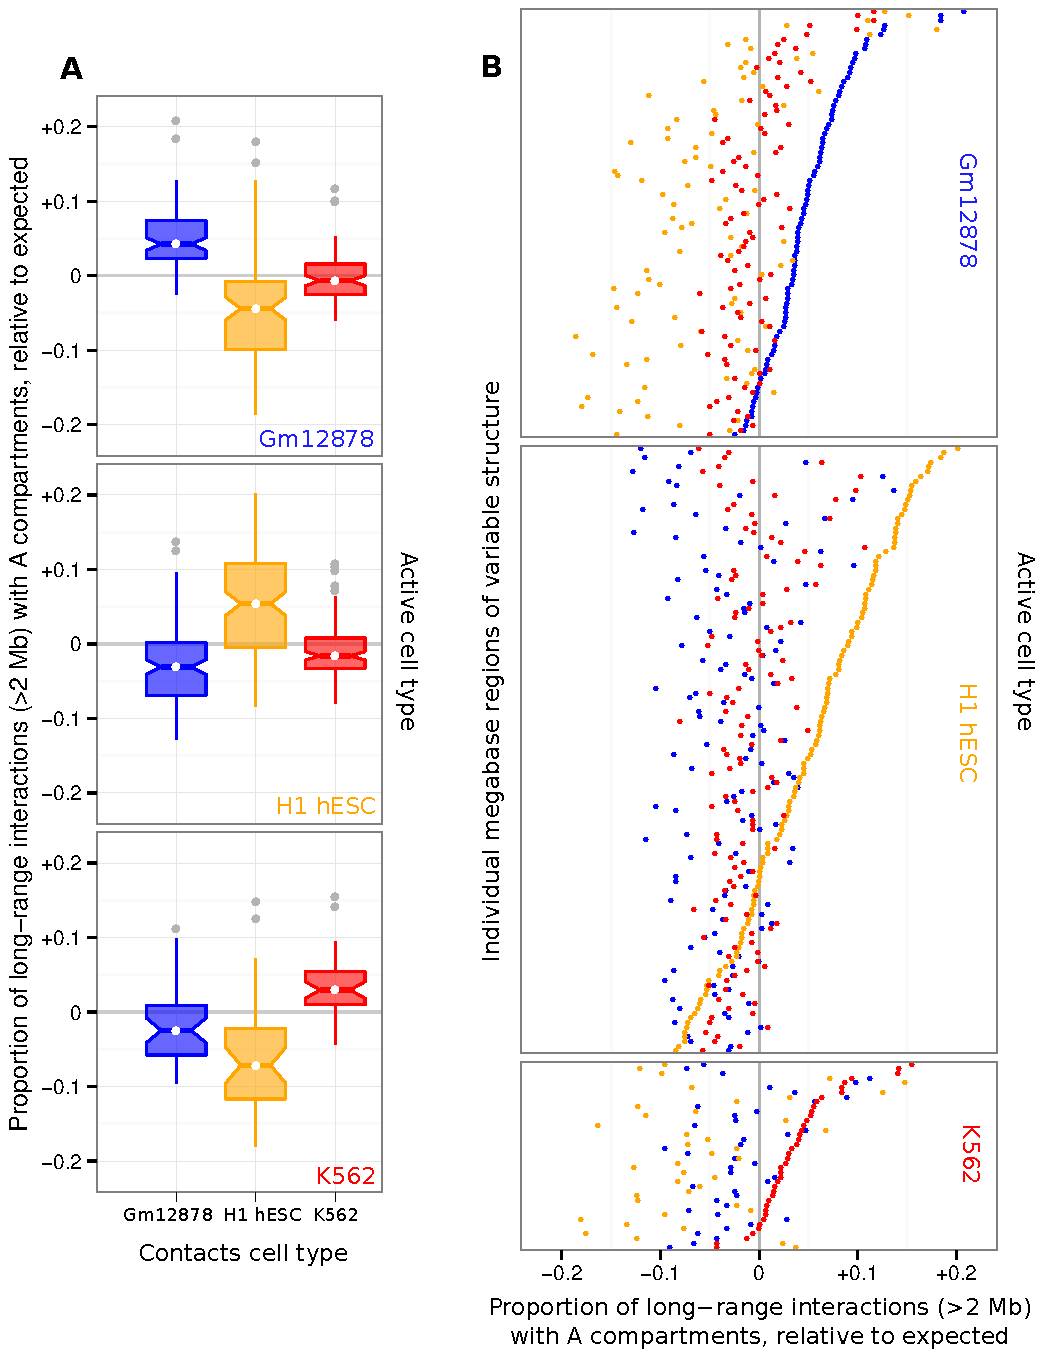
\includegraphics[width=5in]{longrange.pdf}
\captionsetup{width=\textwidth} 
\caption[Regions of variable higher order structure change their genome-wide
contact profiles to favour active compartments.]{ {\bf Regions of variable higher order structure change their genome-wide contact profiles to favour active compartments. }
Genome-wide normalised contacts were summed for each "open" region of variable structure and the relative proportion of those that were with active / A compartments is shown across the three cell types used in this study. Proportions
were subtracted from the genome-wide average per cell type, such that positive values indicate a
greater than expected interaction bias with active compartments. These data are presented both as a summary notched boxplot (A) and with each individual region visualised, sorted by relative proportion of A contacts in active cell type (B). 
}\label{fig:longrange}
\end{center} 
\end{figure} 

% specific example of contact chances, e.g. 4c spider plot / arc diagram

\section{Nuclear positioning}

Chromosome positioning within the nucleus is known to reflect gene density, with the most gene-dense chromosomes occupying the centre of the nucleus in human cells.\cite{Bickmore2013} \citet{Kalhor2012} used a Hi-C variant to recreate probability density maps of chromosome positions which again reflected this feature of higher order chromatin organisation, and also reported active regions were more diffuse than inactive. A testable hypothesis with the eigenvector data used in this work is that active A compartments are enriched in the central nucleus of our human cell types, and B compartments are preferentially located in the nuclear periphery.

To test this, published data on chromosome positioning preference within
the nucleus was used to label chromosomes as ``central'' or 
or ``edge''.\cite{Boyle2001} Chromosomes whose DAPI hybridisation
signals were significantly enriched ($p\leq 2\times10^{-2}$) in the inner nuclear shell, as
defined by \citet{Boyle2001}, made up the ``central''
group and included chromosomes 1, 16, 17, 19 and 22. Similarly the ``edge'' group
had enriched signals ($p\leq 5\times10^{-3}$) in the outer shell relative to the inner nuclear
shell and included chromosomes 2, 3, 4, 7, 8, 11, 13 and 18. The remaining
chromosomes showed no significant preference to either inner or
outer nuclear shells at $\alpha = 0.05$.\cite{Boyle2001} 

We found that positive eigenvectors (reflecting A compartments) did show a modest relative enrichment in centrally-positioned chromosomes relative to those located at the nuclear periphery (Fig. \ref{fig:nucpos}). The significance of this observation was determined by a two-sided Wilcoxon rank sum test on the median eigenvector values of each chromosome, comparing the medians of those chromosomes located in the nuclear periphery and centre (Methods \ref{methods:positioning}). The difference was found to be statistically significant in each case (GM12878: $p < 0.002$; H1 hESC: $p < 0.002$; K562: $p < 0.05$)
%The significance
%of the difference in distribution of eigenvectors in the central
%and edge of the nucleus was determined by a two-sided Kolmogorov-Smirnov (K-S)
%test, with the null hypothesis that there is no difference between the empirical cumulative
%density functions of the central chromosome eigenvectors ($F_{central}$)
%and peripheral ($F_{edge}$). The difference was found to be statistically significant in each cell type ($H_0: F_{edge} = F_{central}$; GM12878: $D = 0.11$, $p < 6 \times 10^{-4}$; H1 hESC: $D = 0.12$, $p < 8 \times 10^{-8}$; K562: $D = 0.10$, $p < 5 \times 10^{-3}$)

\begin{figure}
\begin{center} 
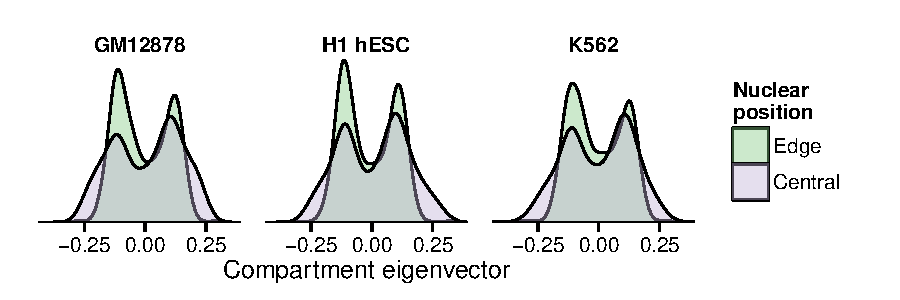
\includegraphics[width=5in]{nucpos.pdf}
\captionsetup{width=\textwidth} 
\caption[Chromosomes located at the nuclear periphery hold a greater proportion of inactive B compartments than those in the central nucleus.]{ {\bf Chromosomes located at the nuclear periphery hold a greater proportion of inactive B compartments than those in the central nucleus. }
Kernel density estimates show the distributions of A (positive eigenvectors) and B compartments (negative eigenvectors) at the edges of the nucleus and at its centre. Positioning data from \citet{Boyle2001} (Methods \ref{methods:positioning}).
}\label{fig:nucpos}
\end{center} 
\end{figure} 


\ifstandalone
\begin{small}
\bibliography{/Users/benmoore/Documents/library,/Users/benmoore/Documents/customrefs}
\end{small}
\fi

\end{document}
